\documentclass[a4paper]{report}

%% Language and font encodings
\usepackage[francais]{babel}
\usepackage[utf8]{inputenc}
\usepackage[T1]{fontenc}
\usepackage{verbatim}

%% Sets page size and margins
\usepackage[a4paper,top=3cm,bottom=2cm,left=3cm,right=3cm,marginparwidth=1.75cm]{geometry}

%% Useful packages
\usepackage{amsmath}
\usepackage{graphicx}
\usepackage[colorinlistoftodos]{todonotes}
\usepackage[colorlinks=true, allcolors=blue]{hyperref}
\usepackage[section]{placeins}
\usepackage{appendix}
\usepackage{nameref}
\usepackage{float}

%% VERY IMPORTANT PACKAGE !!!
\usepackage{fontspec}
%\setmainfont{Dancing Script}	hello debord !

%% For code
\usepackage{listings}
\lstset{
     literate=%
         {à}{{\'a}}1
         {é}{{\'e}}1
         {è}{{\`e}}1
       }

%% Bibliography
\usepackage[bibstyle=numeric, citestyle= numeric,backend=biber,maxbibnames=10]{biblatex}
\addbibresource{bib.bib}
\DeclareNameAlias{sortname}{first-last}
\renewbibmacro{in:}{}

%% For pseudo code
\usepackage{algorithm}
\usepackage[noend]{algpseudocode}
\algrenewcommand\textproc{}% Used to be \textsc


%% For subsubsub...section
%\setcounter{secnumdepth}{5}
\addto\captionsfrench{\renewcommand{\chaptername}{}}

%% For paragraph spacing
\setlength{\parskip}{0.5em}

%%%%%%%%%%%%%%%%%%%%%%%%%%% DOCUMENT %%%%%%%%%%%%%%%%%%%%%%%%%%%%%%%%%%%

\begin{document}
\title{Mémoire}
\author{Emile BARJOU, Christophe CAUBET, Adrien HALNAUT, Romain ORDONEZ}

%
\begin{titlepage}
\centering
{\scshape\LARGE Université de Bordeaux \par}
\vspace{0.75cm}
{\scshape\Large Projet de Programmation 2018\par}
\vspace{1.5cm}
{\Huge\bfseries Jeu de la Guerre\par}
\vspace{0.5cm}
{\Large Mémoire\par}
\vspace{2.5cm}
{\Large\itshape Emile \textsc{Barjou}\par Christophe \textsc{Caubet} \par Adrien \textsc{Halnaut}\par Romain \textsc{Ordonez} \par}
\vfill
Sujet proposé par\par
Philippe {\scshape Narbel}\par
Supervisé par\par
Emmanuel {\scshape Fleury}

\vfill
\end{titlepage}

\vspace*{\fill}
\begin{center}
{\bf Résumé}
\end{center}
Dans ce document, nous détaillerons la manière dont nous avons mené notre Projet de Programmation réalisé dans le cadre de notre première année de Master Informatique à l'Université de Bordeaux.

Ce sujet, proposé par M. Narbel, porte sur la compréhension, puis le développement d'une application permettant de jouer au \textit{Jeu de la Guerre} tel que décrit par Guy Debord.

En vue d'une reprise potentielle du projet, un module d'analyse et une première approche de la réalisation d'un système expert en mesure de décider des coups, pouvant prendre la place d'un joueur réel, sont fournis.

\vspace*{\fill}

\begin{center}
{\bf Abstract}
\end{center}
In this document, we will explain how we led our Programming Project developed in the context of our Master degree in Computer Sciences at the University of Bordeaux.

This subject, given by Mr. Narbel, is about the understanding, and development of an application allowing to play <<\textit{Jeu de la Guerre}>> as described by Guy Debord.

In the perspective of our project being continued, an analysis module and a first approach of the realisation of an expert system able to decide a move, that can replace a real player, are given.

\vspace*{\fill}

%%%%%%%%%%%%%%%%%%%%%%%%%%%%%%%%%%%%%%%%%%%%%%%%%%%%%%%%%%%%%%%%%%%%%%%%%%%%%%%%%%%%%%%%%%%%%%%%%%%%%%%%%%%%%%

%% For paragraph spacing

\chapter*{Remerciements}
\setlength{\parskip}{0.5em}
Nous souhaitons tout d'abord remercier M. Narbel de nous avoir proposé ce sujet, pour son temps et son investissement lors des nombreuses séances de discussions que nous avons pu avoir autour de ce projet. 

Nous remercions aussi M. Fleury, pour son aide et sa patience lors de nos séances de TD ainsi que pour ses conseils avisés qui nous ont grandement aidé à mener à bien ce projet et ce document.

Aussi, nous souhaitons remercier le jury de l'audit, composé de M. Desbarat, M. Mansencal et de M. Lanterne, pour toutes les remarques constructives qu'ils nous ont fourni sur notre présentation et sur l'architecture de notre projet.


\setlength{\parskip}{0.0em}
\tableofcontents

%%%%%%%%%%%%%%%%%%%%%%%%%%%%%%%%%%%%%%%%%%%%%%%%%%%%%%%%%%%%%%%%%%%%%%%%%%%%%%%%%%%%%%%%%%%%%%%%%%%%%%%%%%%%%%
\setlength{\parskip}{0.5em}

\chapter{Introduction}
\section{Domaine}

Le {\it Jeu de la Guerre}\cite{jdg} est un jeu de plateau imaginé par Guy Debord dans son livre éponyme. 

Guy Debord (1931-1994) est un écrivain et philosophe situationniste principalement connu pour son ouvrage {\it Société du spectacle}(1967). Il crée la société "Les Jeux stratégiques et historiques" avec Gérard Lebovici, et imaginent les règles du \textit{Jeu de la Guerre} puis les publient en 1987 dans {\it Le Jeu de la Guerre : Relevé des positions successives de toutes les forces au cours d'une partie}\cite{jdg}.

C'est un jeu au tour par tour qui est centré sur la stratégie militaire et les contraintes auxquelles font face les armées en temps de guerre.
Il oppose deux armées ayant pour objectif de détruire les troupes adverses ou ses moyens de communication. 

Guy Debord s'est inspiré du jeu {\it Kriegsspiel} (voir figure \ref{fig:illu}), crée par Von Reiswitz au XIX\textsuperscript{ème} siècle, qui permet de simuler une guerre entre deux armées permettant d'affiner et de prévoir les tactiques militaires et les affrontements, tout en s'initiant à l'art de la guerre. Ce jeu a été utilisé pendant des décennies par des officiers et commandants, d'abord allemands puis de diverses nationalités, afin de pratiquer des batailles et de prévoir des stratégies d'action. Guy Debord s'est également inspiré de plusieurs des ouvrages de Carl von Clausewitz, dont le plus connu, {\it De la guerre} (ou {\it vom Kriege})\cite{vomkriege}, écrits à la même époque qu'a été crée le {\it Kriegsspiel} de von Reiswitz\cite{kriegsspiel}.

\begin{figure}[H]
\centering
\label{fig:illu}
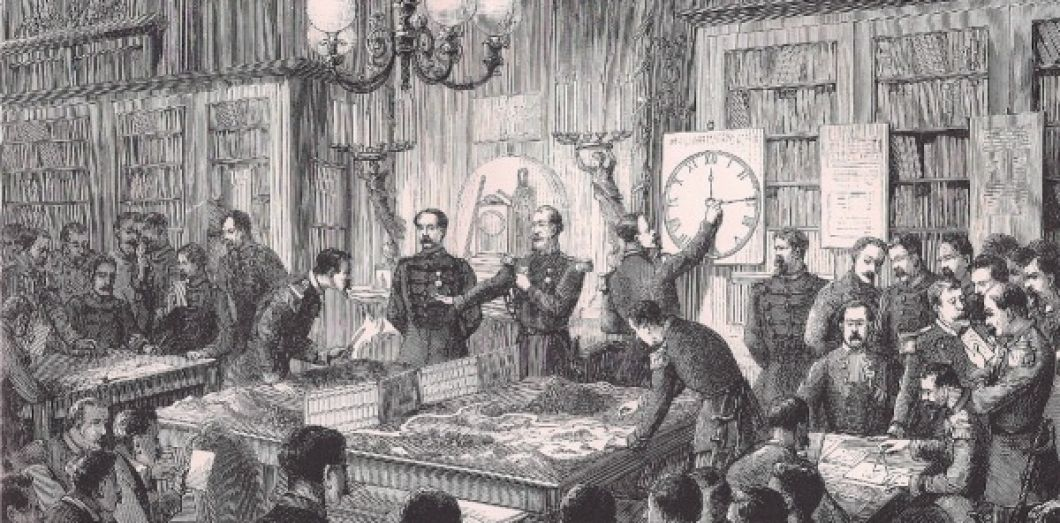
\includegraphics[width=0.8\textwidth]{illujdg}
\caption{"Le Jeu de la Guerre" (Kriegsspiel) dans {\it L'Illustration} du 22 août 1874}
\end{figure}

Les jeux de guerre, ou Wargames, sont le plus souvent des jeux de plateau faisant affronter des camps entre eux pour atteindre un objectif, que ce soit détruire entièrement les effectifs adverses ou bien atteindre une position clé sur le terrain. 
\newpage
De nos jours, ils sont assez répandus, même si la plupart d'entre eux s'adressent à des joueurs confirmés qui veulent principalement rejouer certaines batailles historiques en employant diverses stratégies. On peut notamment citer \textit{DesertFox}, qui permet de rejouer certaines batailles datant de la Seconde Guerre Mondiale en Afrique du Nord, sur un plateau à cases hexagonales. Il est apprécié pour son niveau de complexité et de détails dans la gestion des armées et de la mise en pratique des stratégies.

Ce genre de jeu s'est surtout popularisé grâce à l'arrivée des jeux vidéo qui a permis une simplification dans la gestion des unités et un automatisme dans le calcul de certains mécanismes, l'un des plus répandus est \textit{Civilization} qui met en compétition plusieurs joueurs, automatiques ou non, dans une course à l'expansion dans l'un des domaines permettant la victoire, que ce soit purement militaire ou scientifique et en passant par des victoires plus fines comme religieuse ou politique. Aussi, l'une des particularités de \textit{Civilization} est qu'il joue avec les anachronismes, permettant  de faire affronter Cléopâtre avec Roosevelt sur une carte totalement fictive. 

D'autres jeux, comme la série \textit{Cossacks} ou les \textit{Total War}, ayant un niveau de gestion simplifié mais plus focalisé sur l'aspect militaire, visent le même public que \textit{Civilization}, et d'autres comme la série \textit{Wargame} se rapprochent plus de celui visé par \textit{DesertFox}, mais sans le système de tour par tour.

\section{Sujet}
\label{sec:Sujet}

Ce sujet nous a été proposé par Philippe Narbel, avec qui nous avons pu préciser les besoins autour du projet, et encadré par Emmanuel Fleury avec qui nous avons pu discuter et critiquer nos choix d'implémentations. L'objectif est d'implémenter une version jouable du \textit{Jeu de la Guerre} pour ensuite être en mesure d'analyser une partie.

Il s'agit tout d'abord de comprendre les règles décrites dans l'ouvrage de référence\cite{jdg} pour pouvoir les implémenter dans le moteur de jeu, puis d'ajouter une interface pour rendre le jeu jouable. Enfin, nous devrons extraire des informations pertinentes du jeu qui puissent être utilisées pour élaborer des stratégies, pouvant mener à l'implémentation d'un système expert capable de proposer des coups valides.

Lors de la création de tests, ceux-ci se basant sur des situations présentes dans ce livre, nous nous sommes rendus compte de quelques erreurs d'application des règles. Nous pensons que celles-ci viennent principalement du fait qu'il est assez complexe de décider d'une action dans ce jeu : les joueurs ont pu déplacer des unités pour mieux visualiser leurs actions pendant leur tour, et avant d'effectuer l'action qu'ils allaient réellement jouer, ont pu oublier de replacer correctement leurs unités. Nous pouvons noter une première erreur entre les positions 9 et 9', concernant le tour du camp Sud, où une infanterie se déplace de deux cases arrivant à la case I17, alors qu'elle ne devrait se déplacer que d'une seule case. D'autres erreurs ont été trouvées et répertoriées par Radical Software Games sur leur site Internet\cite{rsgErrata}. Il faudra cependant remarquer que l'erreur soulignée par Radical Software Games à propos de la position 46' de la version 2006 n'en est pas réellement une, car le tour est parfaitement jouable selon les règles du livre.

Étant un point crucial du projet, le moteur de règles doit être entièrement testé pour en garantir sa robustesse et son bon fonctionnement.

\section{Le \textit{Jeu de la Guerre}}

Le projet se base sur le livre\cite{jdg} écrit par Guy Debord, qui est donc notre principale référence, dans lequel est décrit le déroulement complet d'une partie servant d'introduction à son jeu, ainsi que la liste des règles de ce dernier (voir \cite{jdg}, pages 135-160).

C'est un jeu de plateau(\ref{fig:illu_livre}) historique, joué tour par tour, dont le but est de retranscrire les difficultés de mener une bataille, axée sur l'élaboration de stratégies et la mise en place de tactiques.
Le jeu consiste essentiellement à déplacer ses unités et attaquer les unités et bâtiments adverses tout en protégeant les siens.

\begin{figure}[!h]
\centering
\label{fig:illu_livre}
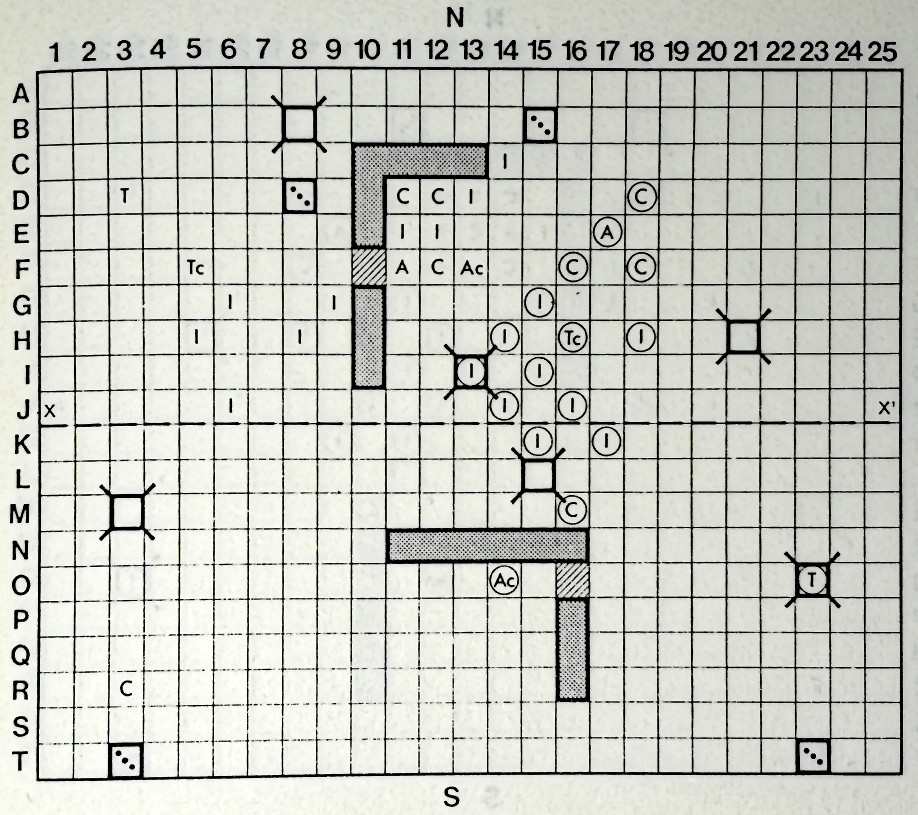
\includegraphics[width=0.8\textwidth]{livre}
\caption{Représentation du plateau de jeu décrit dans le livre du \textit{Jeu de la Guerre}}
\end{figure}

\subsubsection*{\'Eléments du plateau}
Le plateau est composé de cases carrées, 25 de long, et 20 de hauteur, divisé en deux parties égales par une ligne sur le sens de la longueur. Chacune de ces divisions du plateau constitue l'un des deux camps adverses et possède 3 cases forteresses, 2 arsenaux, 9 montagnes et 1 col placé entre deux cases montagnes. Ces éléments ne peuvent se superposer sur une même case. La partie supérieure du plateau représente la zone associée au camp Nord, et la partie inférieure au camp Sud.

Les montagnes ne peuvent pas être occupées ou traversées par une unité, et une attaque ne peut être portée à travers celles-ci.

Les forteresses, ne pouvant être détruites, ainsi que les cols apportent un bonus défensif, respectivement de 4 et de 2, au coefficient de défense aux unités les occupant sans se soucier du côté du terrain où ils sont situés.

Un arsenal est considéré comme détruit lorsqu'une unité combattante du camp adverse a occupé sa case. Aucune unité adverse ne doit être présente sur la case de l'arsenal pour qu'il puisse être détruit.

Chaque camp possède également plusieurs types d'unités, définis par 4 caractéristiques : le coefficient d'attaque, le coefficient de défense, la portée et les points de mouvement.

\subsubsection*{Initialisation de la partie}

Les joueurs doivent disposer ensemble les montagnes et les cols sur le plateau, en respectant les contraintes précédentes. Aussi ces éléments ne doivent pas être disposés de manière symétrique par rapport à la ligne séparant les deux camps.

Les joueurs devront placer leurs bâtiments et leurs unités sur le terrain sans avoir connaissance du placement des effectifs adverses. Les forteresses doivent être posées sur des cases en communication directe (voir section \ref{communicationRules} \nameref{communicationRules}) avec au moins un arsenal allié.
Le joueur qui commence la partie est désigné de manière aléatoire.
 
\subsubsection*{Déroulement d'un tour}
\`A son tour, un joueur peut déplacer jusqu'à 5 de ses unités. Une unité ne peut se déplacer qu'une fois par tour, et elle ne peut se déplacer, attaquer ou défendre que si elle est alimentée en communication. À l'issue de chaque mouvement, le joueur peut attaquer une unité ennemie à portée d'attaque de l'unité qu'il vient de déplacer.

\subsubsection*{Conditions de victoire}
Il existe deux moyens de remporter la victoire, le premier est de détruire les deux arsenaux de l'adversaire, le deuxième est de détruire toutes les unités combattantes adverses.

\subsubsection*{Communications} \label{communicationRules}
Les cases-Arsenal diffusent les lignes de communication dans les 8 directions (horizontales, verticales et diagonales), sans limitation de portée. La diffusion dans l'une des directions est stoppée dès lors qu'elle croise une unité ennemie combattante ou une montagne.

Les unités non-combattantes (les unités relais) alimentées en communication diffusent l'information de la même manière que les arsenaux. Les unités combattantes alimentées en communication diffusent l'information sur leurs 8 cases adjacentes, les unités se trouvant sur ces cases diffusent à leur tour l'information.

\subsubsection*{Attaquer et défendre}
  \begin{itemize}
    \item L'attaque se déroule sur une case définie par le joueur attaquant, à savoir la case où se trouve l'unité attaquée.
    \item Toutes les unités du joueur à portée d'attaquer cette même case additionnent leurs coefficients offensifs. Les unités du joueur défendant à portée d'attaquer cette même case additionnent leurs coefficients défensifs.
    \item Le résultat de la soustraction des coefficients offensifs par les coefficients défensifs permet trois situations :
    	\begin{enumerate}
          \item Le résultat est inférieur ou égal à 0, il ne se passe rien.
          \item Le résultat est supérieur ou égal à 2, l'unité attaquée est détruite.
          \item Le résultat est égal à 1, lors du prochain tour, l'adversaire devra, avant toute autre action, utiliser un de ses coups pour déplacer l'unité attaquée vers une case vide. Cette unité ne pourra participer à aucune offensive pendant ce prochain tour.
    	\end{enumerate}
        \item Une unité ayant attaqué ne peut plus se déplacer jusqu'à la fin du tour.
        \item Une unité de cavalerie peut, à l'issue de son déplacement, initier une charge contre une unité ennemie se trouvant sur une des 8 cases adjacentes à une unité de cavalerie. Cette unité peut être la même que celle qui initie l'attaque, et doit se trouver sur l'axe reliant l'unité attaquée et celle attaquante sans discontinuité de cases entre elles. La charge donne un coefficient offensif de 7 à cette unité de cavalerie, et permet de faire participer à l'offensive les autres unités de cavalerie alliées se trouvant dans le même alignement de cases sans discontinuité de cases entre elles. Ce faisant, les unités de cavalerie participant à la charge voient leurs coefficients offensifs montés à 7 (voir figure \ref{fig:help_charge}). 
        
\begin{figure}[H]
\centering
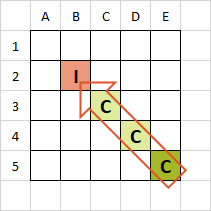
\includegraphics[width=0.30\textwidth]{help/charge}
\caption{Exemple d'une charge de 3 cavaliers sur l'unité en B2 initiée par le cavalier en E5}\label{fig:help_charge}
\end{figure}
        
        \item Une charge ne peut être initiée contre une unité se situant sur un col de montagne ou dans un fort, et une unité se situant dans un fort ne peut y participer.
        \item La prise et destruction d'un arsenal ennemi est considérée comme une attaque, et l'unité à l'origine de cette prise ne peut donc pas initier d'offensive à l'issue de son déplacement.
    \end{itemize}

%%%%%%%%%%%%%%%%%% EXISTANT %%%%%%%%%%%%%%%%%%%%%%%%%%%%%%%%%%%%%%%%%%

\chapter{Existant}
\section{Assimilation du sujet et prototype}

Les règles de ce jeu demandant un peu de temps à bien être comprises, nous avons décidé de faire quelques parties avant de se lancer dans le développement du programme, nous permettant de mieux comprendre les mécanismes du jeu et les enjeux stratégiques derrière celui-ci.

Cependant, nous nous sommes rendus compte assez vite qu'il n'existait pas de support jouable, ni plateau réel ou même virtuel. Nous avons donc décidé de faire un prototype papier (voir figures \ref{fig:plateau_irl} et \ref{fig:plateau_irl2}).


\begin{figure}[h]
\centering
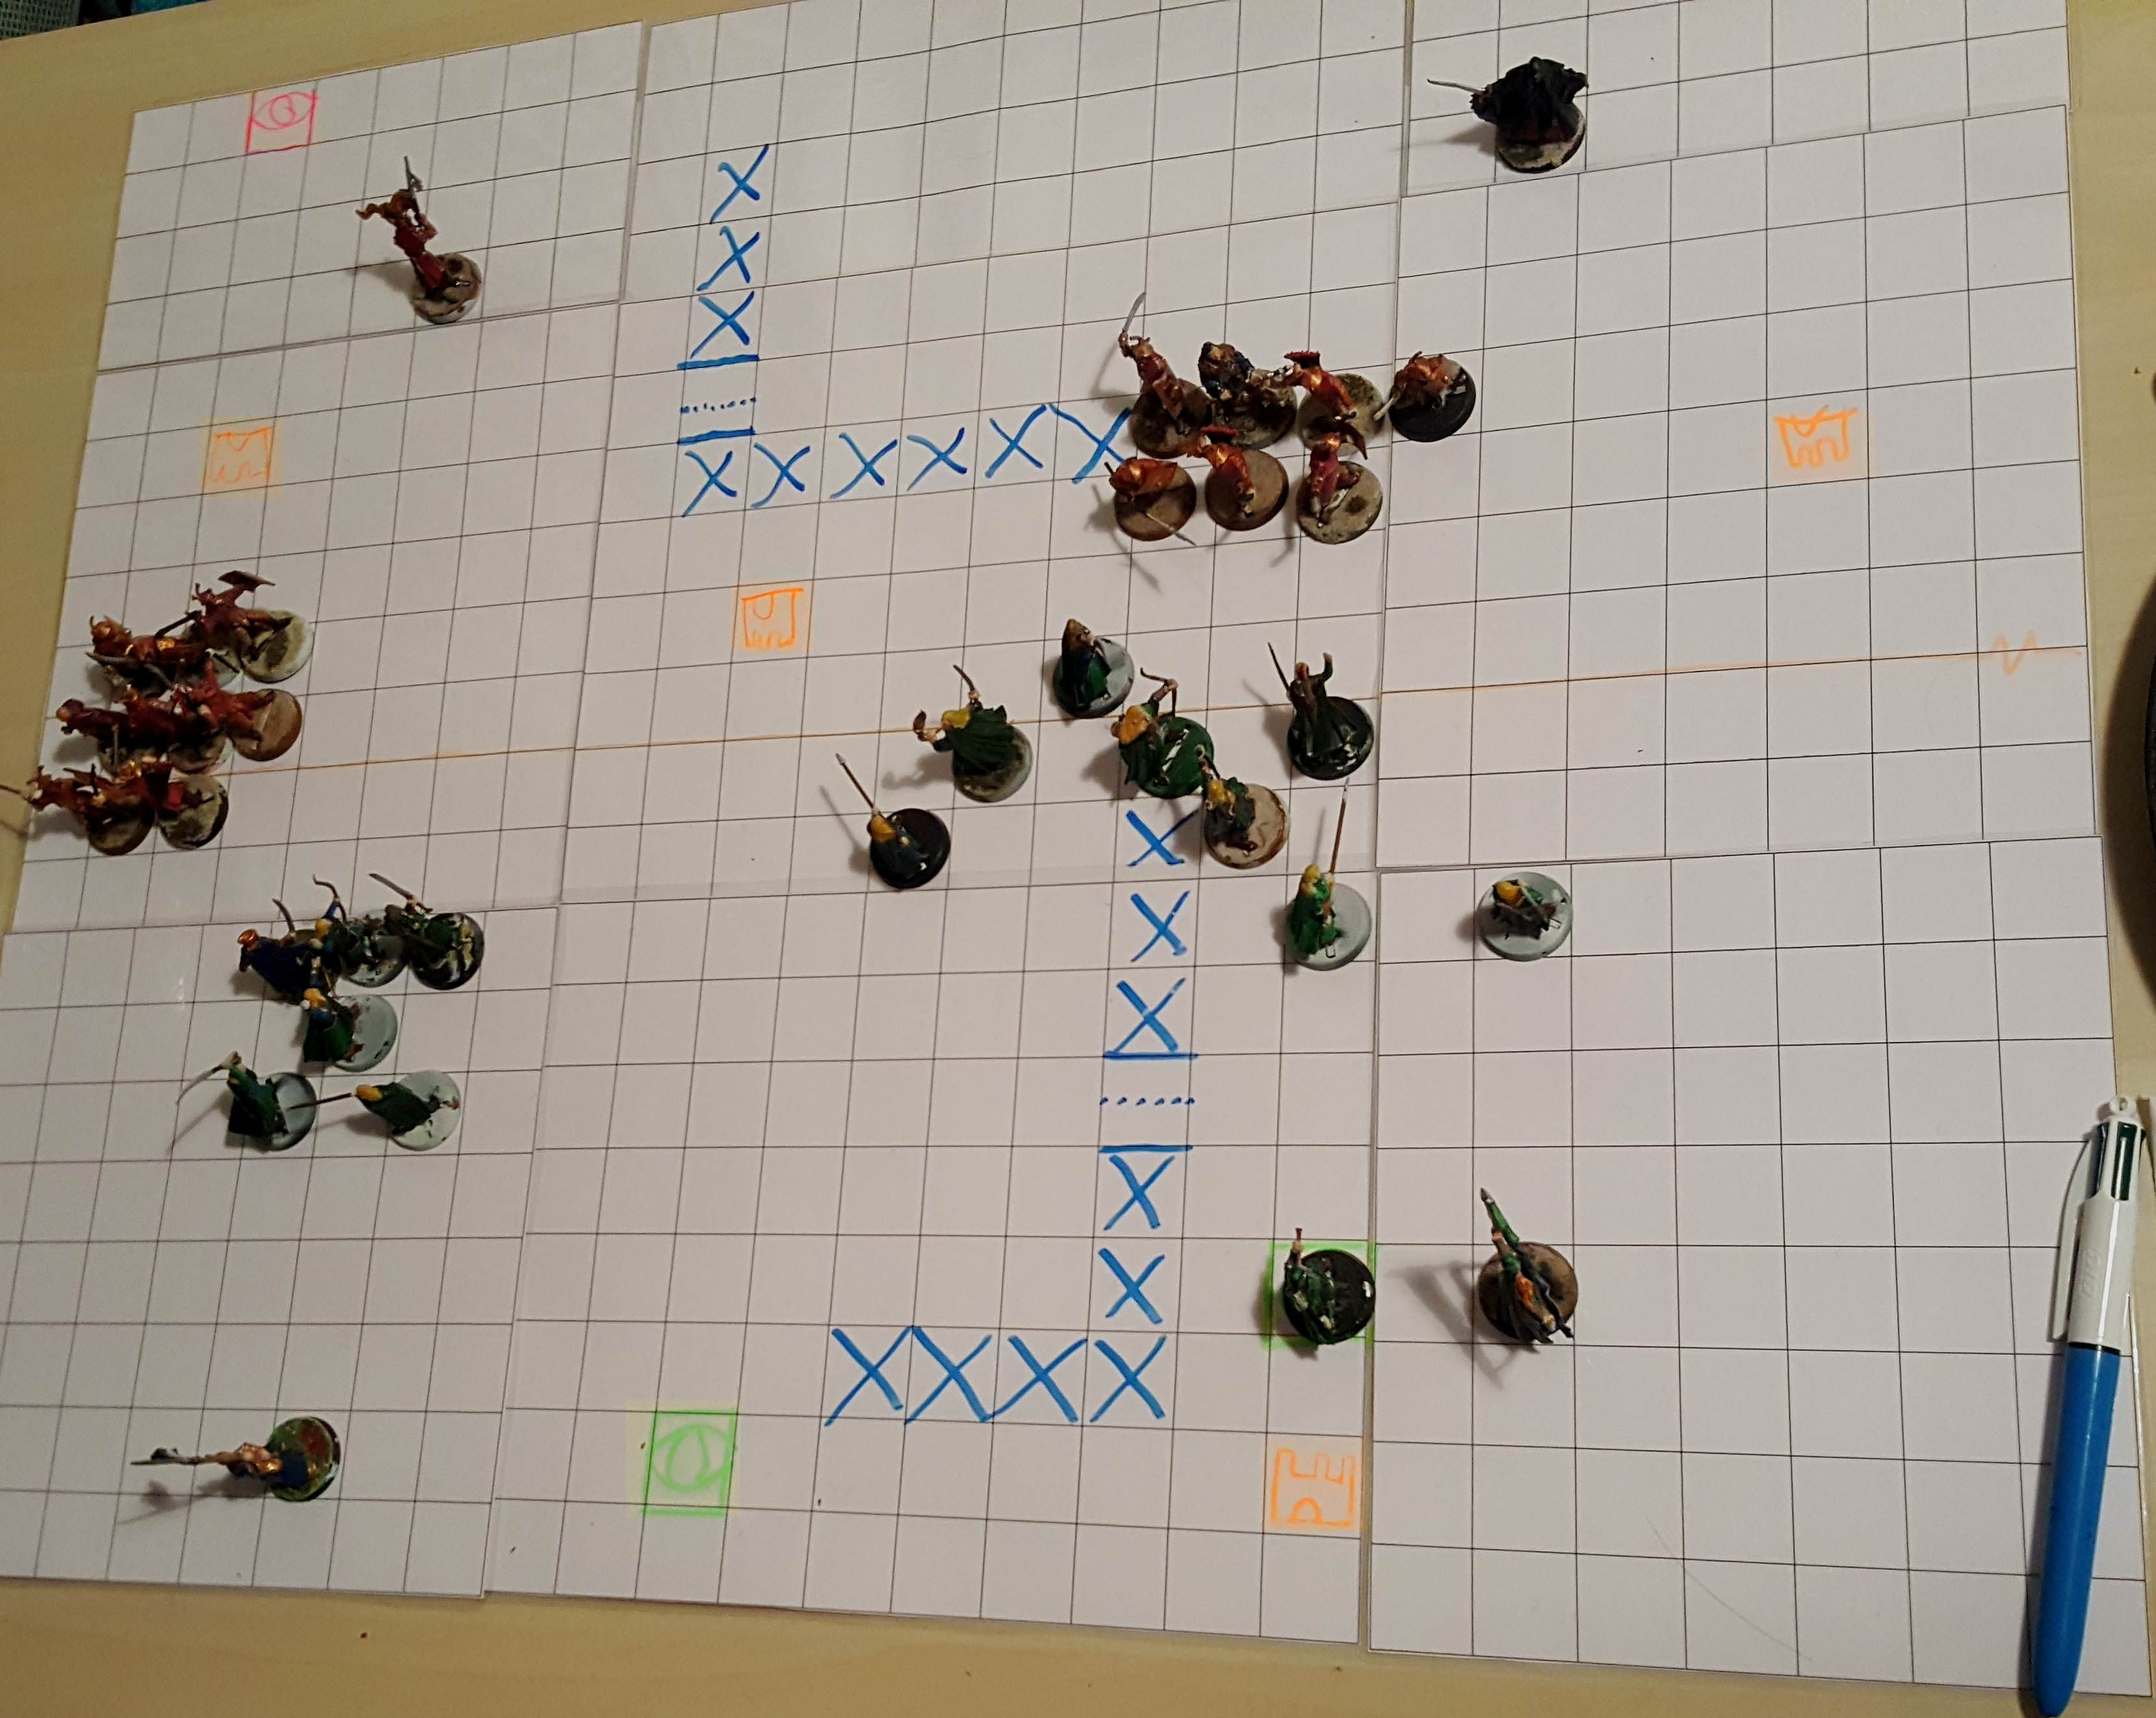
\includegraphics[width=0.84\textwidth]{existantPlateau/plateau2}
\caption{Prototype papier du {\it Jeu de la Guerre}}\label{fig:plateau_irl}
\end{figure}


Cette version nous a permis de découvrir la dimension tactique du jeu et que certains positionnements d'unités, notamment un groupe de 5 unités "en étoile" (Vu en détail en section \ref{sec:analyseEtoile} \refname{sec:analyseEtoile}), sont plus efficaces que d'autres dans l'optique de conserver un maximum de potentiel d'attaque et de défense tout en avançant vers les lignes adverses. Nous nous sommes également rendus compte lors de ces parties que nous passions la majeure partie du temps à vérifier l'alimentation des communications et à calculer les valeurs d'attaque et de défense.

\begin{figure}[h]
\centering
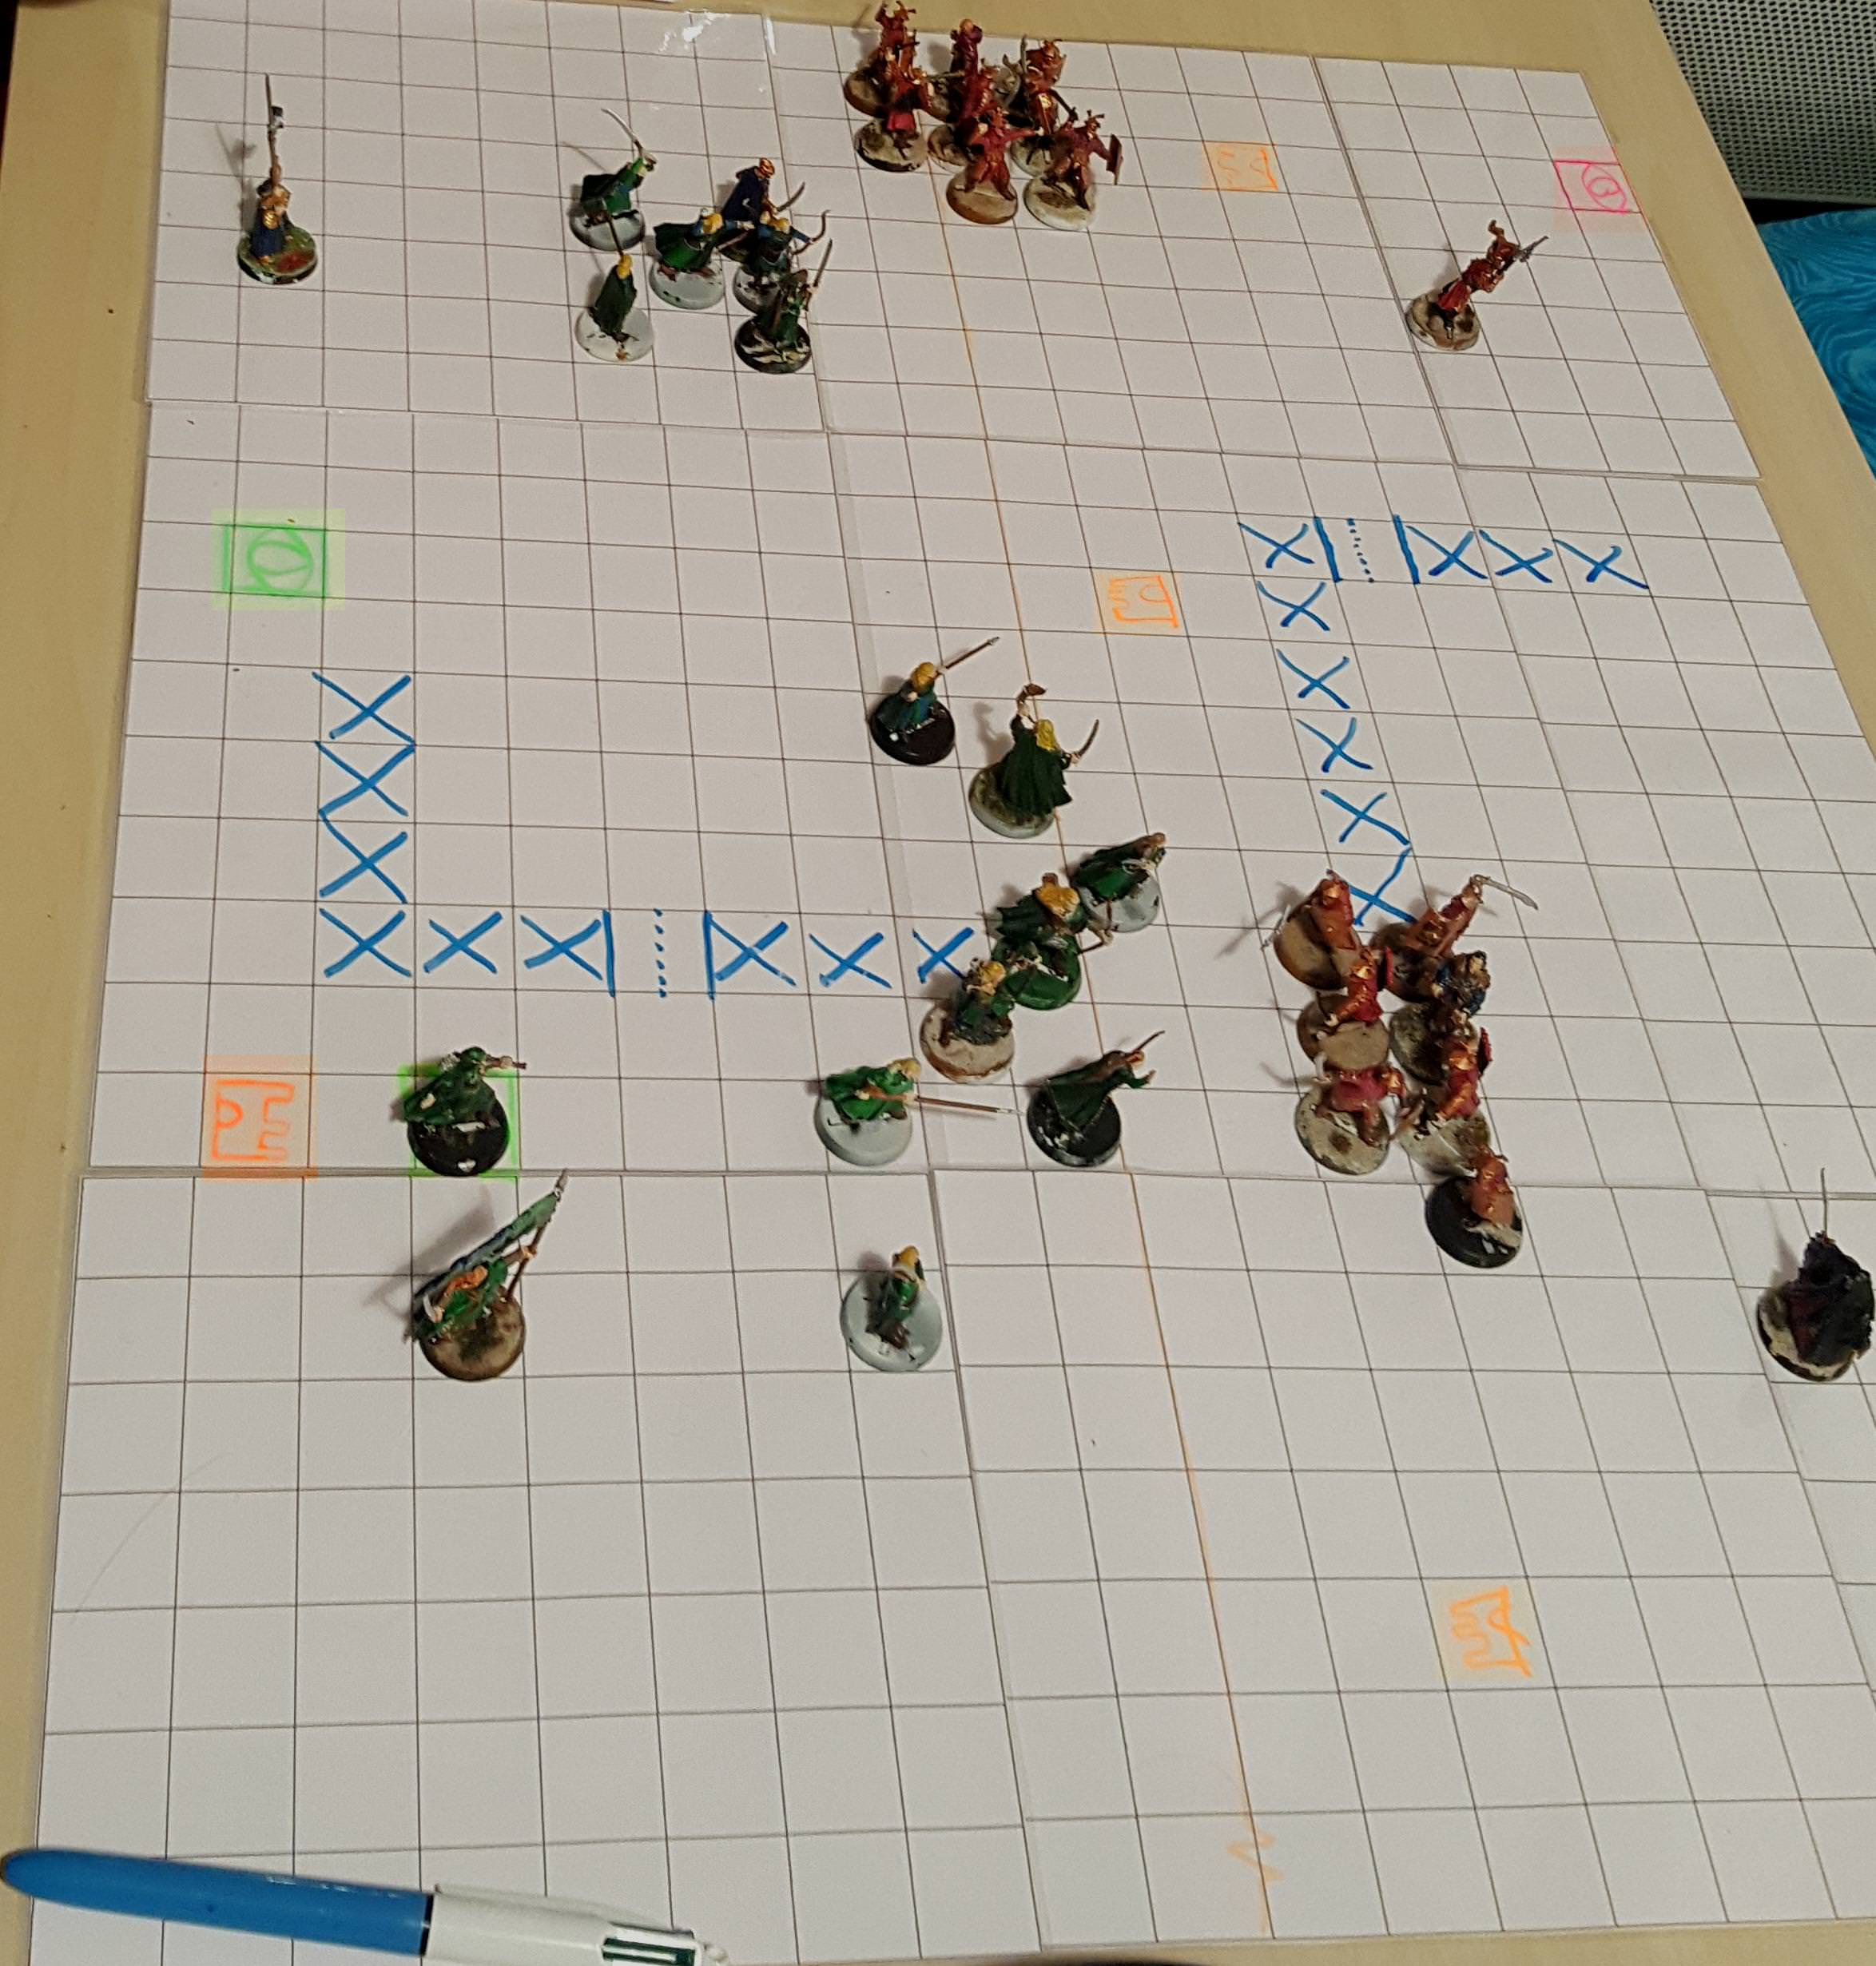
\includegraphics[width=0.85\textwidth]{existantPlateau/plateauMaison}
\caption{Prototype papier du {\it Jeu de la Guerre} - autre point de vue}\label{fig:plateau_irl2}
\end{figure}

\section{Autres projets}

Il existe d'autres projets autour du \textit{Jeu de la Guerre}, l'un d'entre eux venant d'un ancien projet de programmation dans le cadre de cette UE.


\subsection*{PdP 2014}
Ce projet\cite{pdp2014} permet la visualisation d'une instance d'une partie sans interaction possible avec le plateau. L'interface permet la visualisation des lignes de communication (voir figure \ref{fig:PdP2014Com}), la portée de déplacement d'une unité ainsi que le potentiel offensif (voir figure \ref{fig:PdP2014Atk}) et défensif (voir figure \ref{fig:PdP2014Def}) de chaque camp pour chaque case du plateau.
Ce projet nous a donné des idées de fonctionnalités à implémenter concernant l'interface graphique pour l'utilisateur. 


\begin{figure}[H]
\centering
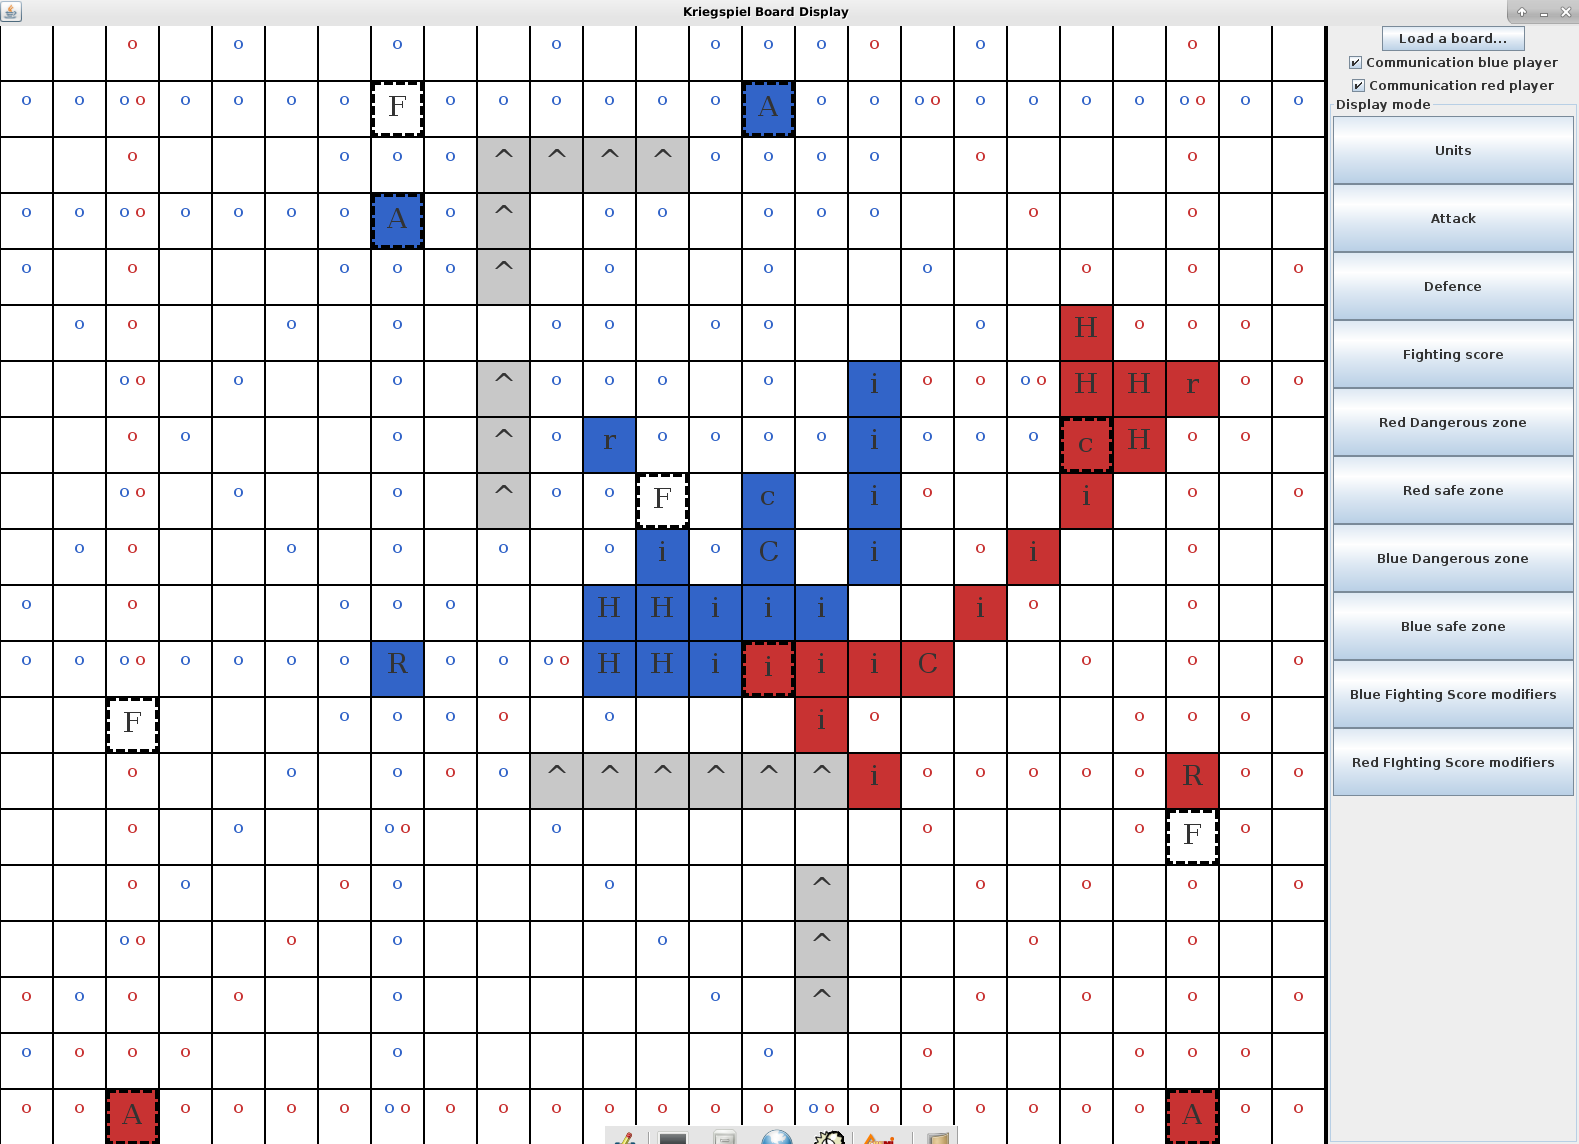
\includegraphics[width=0.8\textwidth]{existantPDP/pdp2014}
\caption{Capture d'écran du programme développé du PdP 2014}\label{fig:PdP2014Com}
\end{figure}


\subsection*{\textit{Kriegspiel} par Radical Software Games\cite{rsg}}
Ce projet n'est plus disponible sur le site de Radical Software Games, mais nous disposons grâce à M. Narbel des sources du jeu. Il permettait de jouer en réseau contre un autre joueur au \textit{Jeu de la Guerre} avec des règles simplifiées. Des aides visuelles sont présentes sur le plateau du jeu, permettant de voir les lignes de communication de chaque camp, les cases où peuvent se déplacer les unités et si ces cases sont à portée d'une ligne de communication (fig. \ref{fig:jdgRSG}). Il semble bien fonctionnel, mais a été retiré du site depuis. Il semblerait que ce soit la veuve de Guy Debord, Alice Becker-Ho, qui soit à l'origine du retrait\cite{finmot-rsg} du jeu.

Cependant, selon un article datant de 2011 de \textit{l'Express} \cite{bnfDebord}, les archives de Guy Debord sont désormais la propriété de la Bibliothèque Nationale de France.

\begin{figure}[H]
\centering
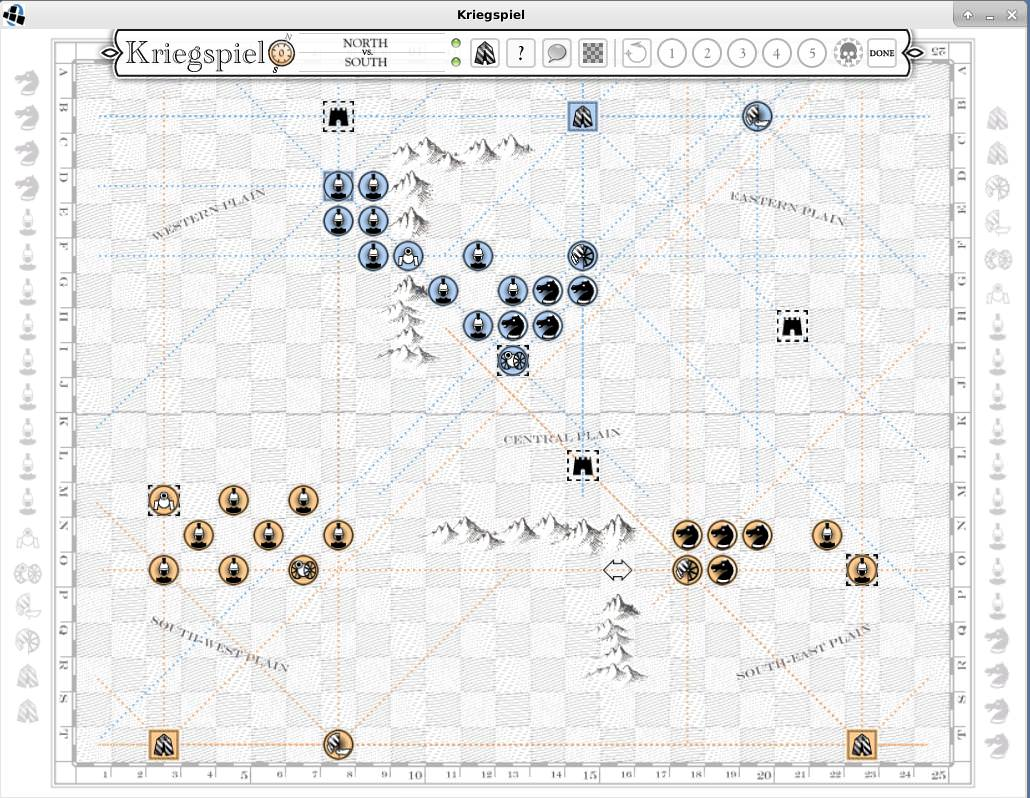
\includegraphics[width=0.9\textwidth]{existantRSG/rsg}
\caption{Interface de \textit{Kriegspiel} par Radical Software Games}\label{fig:jdgRSG}
\end{figure}

\subsection*{Conclusion}
\`A notre connaissance, et après des recherches, nous pensons donc qu'il n'existe pas de version jouable du \textit{Jeu de la Guerre} actuellement disponible. Cependant, il existe d'autres jeux semblables au jeu de Debord partageant le principe de simuler une guerre sur un plateau afin de revivre des batailles historiques et/ou de comprendre les tactiques derrière ces affrontements. On peut notamment citer \textit{DesertFox}\cite{desertfox} qui était à l'origine le jeu proposé pour ce sujet, mais d'une complexité bien supérieure à celle du \textit{Jeu de la Guerre}. Nous avons donc dû créer les bases de notre projet, mais les projets que nous avons cité nous ont tout de même servi dans notre réflexion sur comment mener à bien le notre, ainsi que sur quelques pistes notamment pour concevoir l'interface utilisateur.



\begin{figure}[h]
\centering
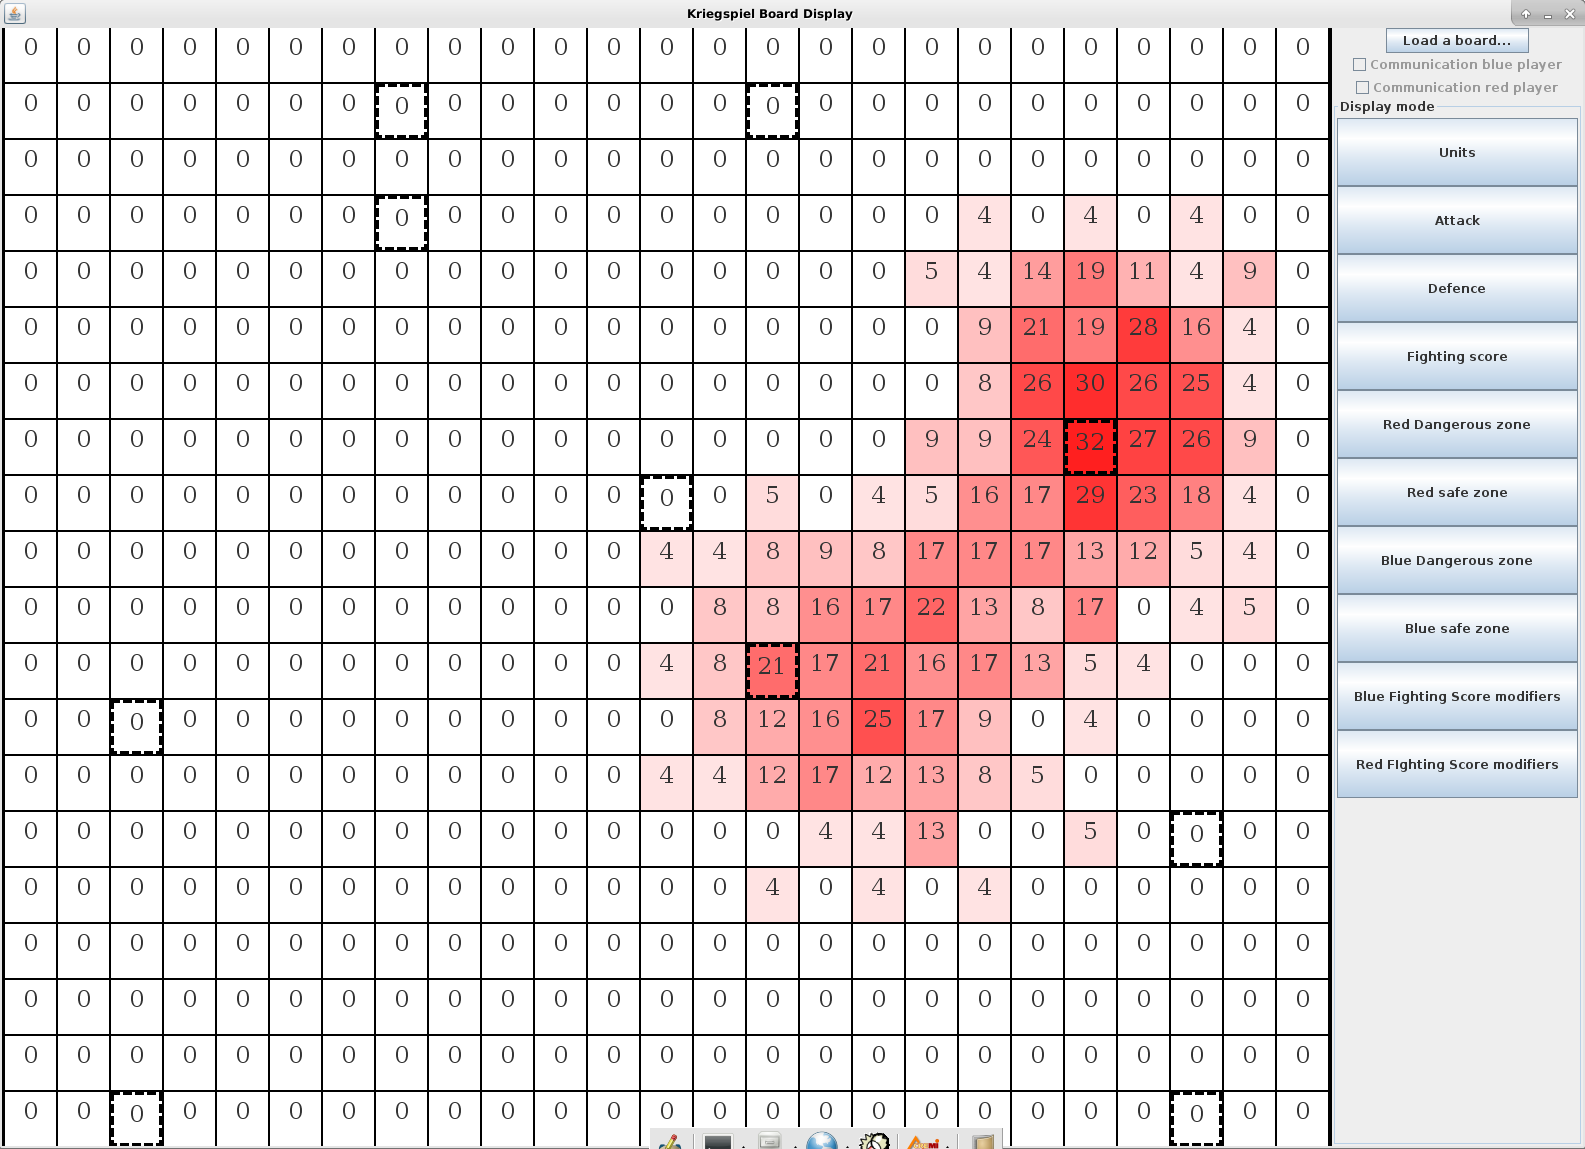
\includegraphics[width=0.8\textwidth]{existantPDP/pdp20142}
\caption{Potentiel d'attaque des unités rouges (PdP 2014)}\label{fig:PdP2014Atk}
\end{figure}

\begin{figure}[h]
\centering
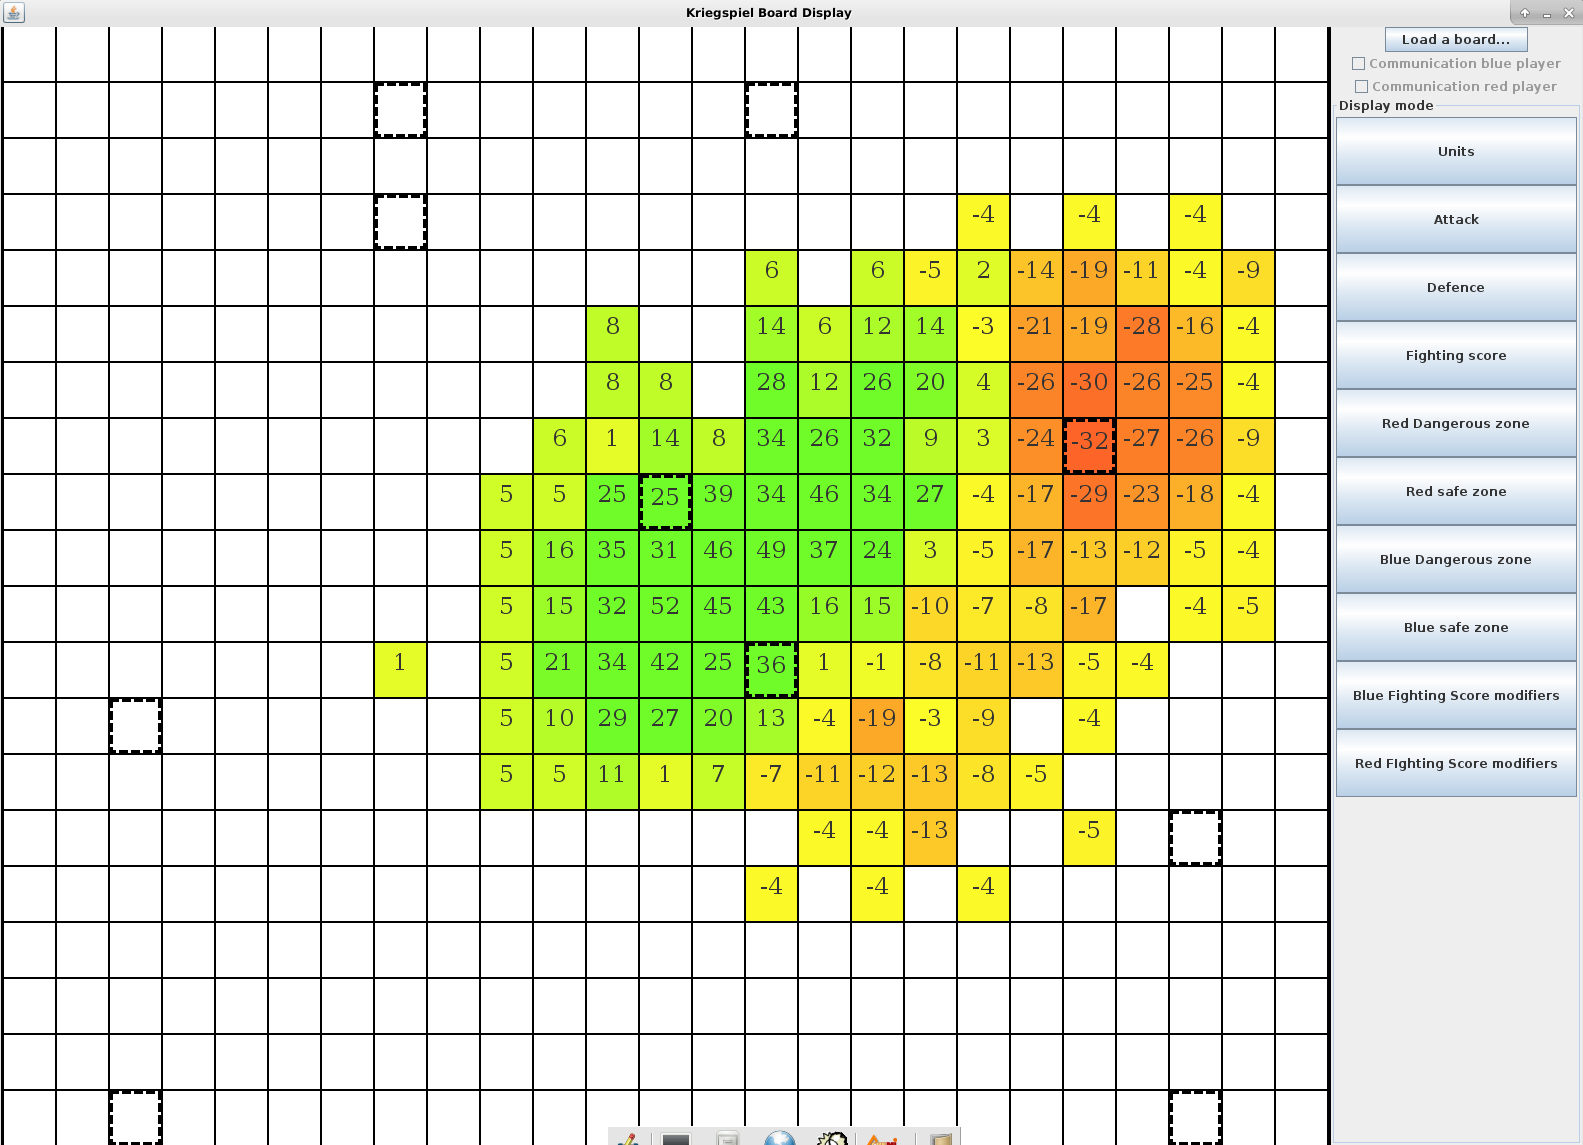
\includegraphics[width=0.8\textwidth]{existantPDP/pdp20143}
\caption{Variation de potentiel de défense des unités bleues (PdP 2014)}\label{fig:PdP2014Def}
\end{figure}


%%%%%%%%%%%%%%%%% Cahier des besoins %%%%%%%%%%%%%%%%%%%%%%%%%%%%%%%%%%%%%%%%%%%

\chapter{Cahier des besoins}

La liste des besoins et leur ordre de priorité ont été établis avec le client M. Narbel et nous avons déterminé trois niveaux de besoins : primaire, secondaire et tertiaire.

Les besoins primaires sont la liste des services que notre programme doit impérativement fournir pour le rendu final du projet et qui doivent être testés au maximum pour en garantir la robustesse de l'implémentation.

Nous devons également implémenter les besoins secondaires autant que possible, ou à défaut en faciliter l'implémentation pour une possible reprise du projet.
Enfin, les besoins tertiaires sont des pistes d'évolutions qui ne seront pas nécessairement finalisés, mais l'architecture du projet doit être adaptée à leur ajout.

\section{Besoins primaires} % Priorité 0

\begin{enumerate}

\item Lire les commandes écrites par l'utilisateur dans un champ de saisie de texte et les traduire en coup (Détaillé en figure \ref{fig:commands}):
	\begin{itemize}
    \item La position de chaque case est décrite par l'utilisateur à l'aide d'une ou plusieurs lettres suivies, sans espace, d'un nombre représentant respectivement l'axe des ordonnées et des abscisses. Ainsi, la case supérieure gauche est A1 et la case inférieure droite est T25.
	\item Déplacer une unité sur une case ciblée vers une autre case : \texttt{move <C1> <C2>} où \texttt{C1} est la case de l'unité alliée ciblée, \texttt{C2} la case d'arrivée
    \item Attaquer une case en ciblant la case de l'unité attaquante : \texttt{attack <C1> <C2>} où \texttt{C1} est la case de l'unité alliée ciblée, \texttt{C2} la case où se situe l'unité ennemie attaquée.
    \item Déclarer la fin de son tour : \texttt{end}
	\end{itemize}

\item Vérifier qu'un coup est valable pour l'état de jeu actuel à l'aide d'un moteur de règles implémentant celles décrites dans le livre \textit{Jeu de la Guerre}.
	\begin{itemize}
    \item Vérifier que la commande est bien demandée par le joueur dont c'est le tour.
    \item Vérifier que le joueur peut encore effectuer des actions pendant ce tour.
    \item Vérifier les règles spécifiques aux mouvements et attaques.
    \item Vérifier qu'une retraite ne doit pas être réalisée avant tout autre coup.
	\end{itemize}
    
\item Appliquer un coup validé en modifiant l'état de jeu actuel.
    
\item Simuler un coup sur une instance d'un plateau sans le modifier pour aider un joueur automatique.

\item Permettre à deux utilisateurs de jouer sur une même interface graphique à tour de rôle.

\item Afficher l'état du plateau actuel, comprenant les unités et les bâtiments à l'aide d'icônes différentiables. (voir figure \ref{fig:prerelease})

\item Afficher le joueur dont c'est le tour.

\item Afficher le nombre de coups restant au joueur ce tour-ci.

\item Déterminer et afficher les informations de fin de partie et du vainqueur.

\end{enumerate}

\section{Besoins secondaires} % Priorité 1

\begin{enumerate}
\item Lorsqu'un coup est refusé par le moteur de règles, afficher une explication du refus.

\item Générer par un clique gauche, dans la ligne de commande, les coordonnées correspondant à la case cliquée par l'utilisateur dans le format attendu par le jeu.

\item Sauvegarder l'état du plateau dans un fichier texte, en codage ASCII, en respectant un ordre logique des informations stockées, le fichier sera lisible par l'utilisateur, dans le format détaillé en figure \ref{fig:savefile}. Cette action sera possible à l'aide de la commande : \texttt{save <file>}. Un exemple d'un tel fichier est donné en annexe \ref{lst:formatDebord}.

\begin{figure}[!h]
\caption{Format du fichier de sauvegarde}
\label{fig:savefile}
\centering
\begin{lstlisting}[basicstyle=\scriptsize\tt, columns=fullflexible]
<Largeur>;<Hauteur>
<Joueur actuel>;<Nombre de coup restant>
<ID d'un terrain>;<X>;<Y>;<Joueur>
...
<ID d'une unité>;<X>;<Y>;<Prioritaire ?>;<Peut bouger ?>;<Dernière unité déplacée ?>;<Peut attaquer ?>;<Joueur>
...
\end{lstlisting}
\end{figure}

\item Instancier une partie à partir d'un fichier texte valide, en codage ASCII, respectant l'ordre et la syntaxe décrits par la sauvegarde. Cette action sera possible à l'aide de la commande : \texttt{load <file>}.

\item Annuler la dernière action effectuée par l'utilisateur à l'aide de la commande : \texttt{revert}.

\item Extraire des informations sur l'état du jeu telles que les lignes de communications, la carte des potentiels d'attaque, de défense ou de déplacement.

\item Afficher sur le plateau des aides visuelles à l'aide de couleurs pour mettre en avant les informations extraites.

\item Choisir quel type et de quel joueur afficher les informations à l'aide d'un menu.

\item Afficher une légende des unités et bâtiments, comprenant leurs icônes et leurs attributs.

\item Pouvoir positionner sur le plateau les unités à l'aide d'une commande dédiée lors de la phase de positionnement des unités.

\item Pouvoir remplacer un joueur humain par un joueur automatique pouvant générer des coups pendant son tour.

\end{enumerate}

\section{Besoins tertiaires} % Priorité 2

\begin{enumerate}

\item Évaluer ("Comprendre") une situation du jeu à un moment donné,
   (Spatial Reasoning\cite{spatial-reasoning} - Potential fields - PathFinding)
   Détermination de "points décisifs".
   
\item Fournir une représentation visuelle de ces évaluations en plus des informations extraites du jeu.

\item Évaluer ("Comprendre") une situation du jeu sur quelques coups ou tours.
   Prise en compte de techniques de planification (Planning).
   Représentation graphique de cette évaluation.

\item Élaborer et mettre en place une stratégie permettant de trouver le chemin le plus efficace pour atteindre les arsenaux de l'adversaire (analyse des "vallées" ou faiblesses dans la formation adverse pour atteindre l'objectif).

\item Élaborer et mettre en place une tactique permettant d'obtenir une configuration optimale dans la planification d'une attaque ou d'une défense (utilisation d'une cartographie des potentiels d'attaque et de défense).

\end{enumerate}



\begin{figure}[h]
\centering
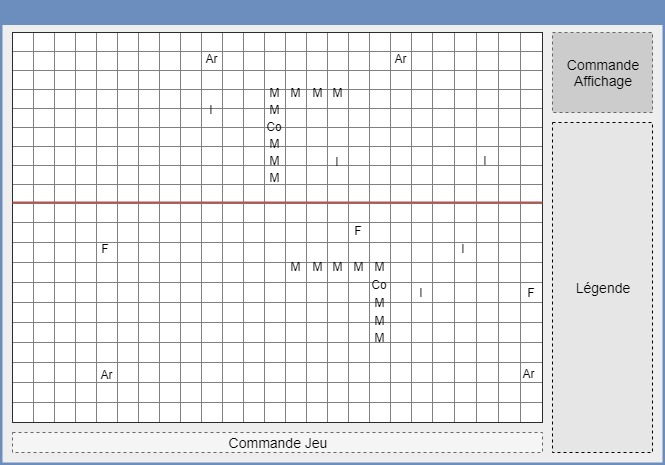
\includegraphics[width=0.8\textwidth]{ui_maquette}
\caption{\'Ebauche d'interface commande et d'aperçu de l'état du plateau}
\label{fig:prerelease}
\end{figure}

\begin{figure}[h]
\centering
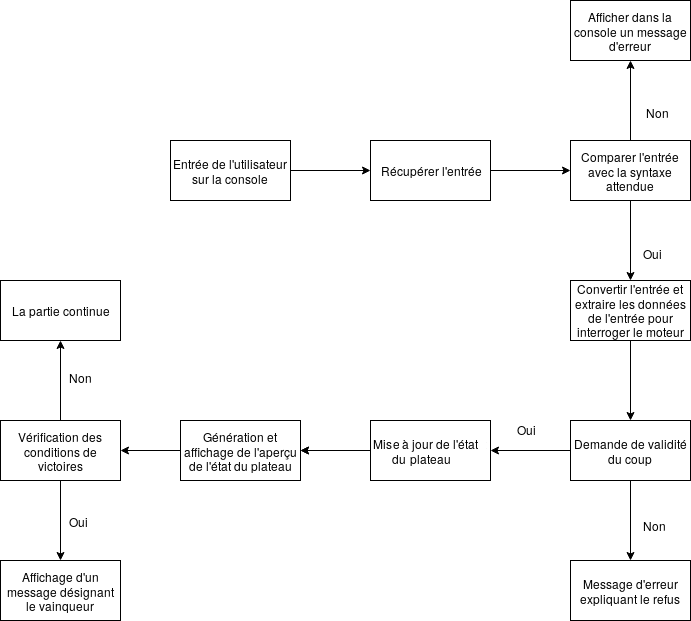
\includegraphics[width=1\textwidth]{scenario}
\caption{Scénario d'utilisation pour un coup proposé}
\label{fig:scenario1}
\end{figure}

\section{Besoins non-fonctionnels}

\begin{enumerate}
\item Le code du moteur de règles devra avoir un certain degré de généricité et de modularité pour pouvoir altérer les règles du jeu.

\item Le temps d'attente entre un coup proposé et sa validité évaluée par le moteur de règles devra être de l'ordre de la seconde.

\item Le jeu doit fonctionner sur un système UNIX.

\item Le jeu sera codé dans le langage de programmation Java.

\item Une couverture des tests sur les différents modules du jeu est attendue lors du développement. Ces tests devront être implémentés par les développeurs travaillant sur leurs modules au fur et à mesure.

\item Les actions de déplacement, d'attaque et de fin de tour devront être testées, aussi bien pour des actions valides qu'invalides, pour une instance du plateau donnée. De plus, certains de ces tests devront inclure des instances continues de la partie de Guy Debord où le mécanisme testé est présent.

\item Des tests en boîte noire devront être fournis, permettant de valider les interactions entre l'utilisateur et le programme. Certains de ces tests se baseront sur les configurations du plateau de la partie décrite dans le livre de Debord (voir \cite{jdg}, pages 14-24), notamment pour vérifier si l'état du plateau résultant du test sur l'état initial est bien conforme à ce qui est décrit. Cette partie servira aussi de témoin principal pour confirmer la validité des règles implémentées.

\end{enumerate}

%%%%%%%%%%%%%%%%%%% PRESENTATION LOGICIEL%%%%%%%%%%%%%%%%%%%%%%%%%%%%%%%%%%%%%%%%%%%
\chapter{Présentation du logiciel}
\section{Interface}
Le logiciel se présente sous la forme d'une fenêtre graphique (voir figure \ref{fig:presui}) comprenant l'affichage du plateau de jeu, un champ de texte pour y entrer les commandes, une légende et un menu pour indiquer quel type d'information afficher sur le plateau (par exemple les lignes de communications, les potentiels d'attaque ou de défense, voir section \ref{sec:analyse} \nameref{sec:analyse}).

\begin{figure}[h]
\centering
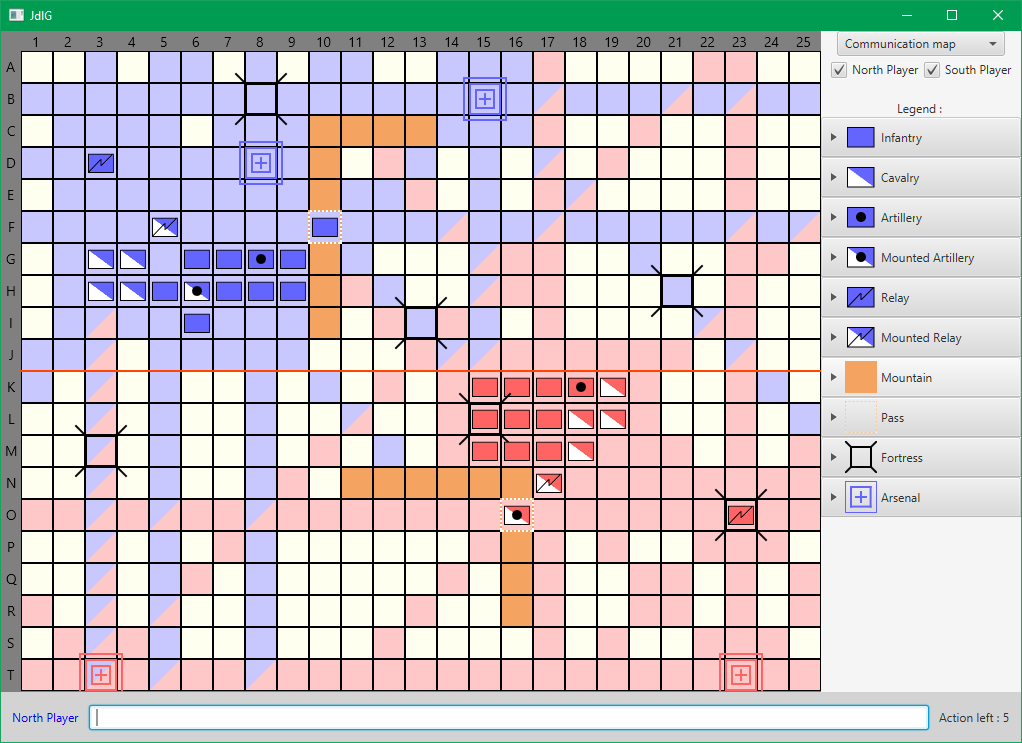
\includegraphics[width=1.0\textwidth]{interface/ui_full_com}
\caption{Interface graphique du logiciel}\label{fig:presui}
\end{figure}

Le plateau est la partie centrale de la fenêtre, et est redessiné dynamiquement lors du redimensionnement de celle-ci. Dessus y sont dessinées les cases avec leurs unités et bâtiments, et l'information choisie (par défaut les lignes de communications).

La barre de commande sur la partie inférieure de la fenêtre comporte, en plus du champ de texte, le nom du joueur auquel c'est au tour de jouer et du nombre de coups qu'il lui reste.

Enfin le panneau latéral comporte en haut le menu déroulant pour l'information ainsi que deux cases à cocher pour choisir de quel joueur afficher cette information. En dessous se trouve la légende faisant correspondre les unités et leurs icônes, qui peut être étendue pour afficher les informations relatives à l'unité.

Lors du lancement du logiciel, la partie commence directement, dans la configuration initiale de la partie du livre de référence.

\begin{figure}[h]
\centering
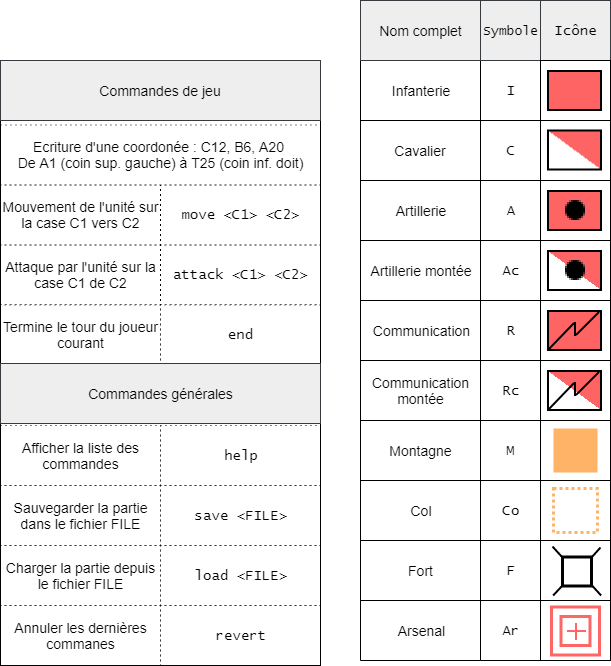
\includegraphics[width=0.8\textwidth]{interface_pdp}
\caption{Commandes et identifiants des unités et terrains employés}
\label{fig:commands}
\end{figure}

\section{Commandes}
%% Une configuration différente peut être chargée par la commande {\tt load} (Format du fichier détaillé en \ref{fig:savefile}).
%% La liste complète des commandes se trouve dans le chapitre du cahier des besoins (\ref{fig:commands}). La commande '\texttt{help}' fournit également la liste des commandes actuellement disponibles. 
%% Les commandes pour jouer sont '{\tt move}' (ou '{\tt m}') et '{\tt attack}' (ou '{\tt a}'). Toutes les actions du jeu pourront se faire à travers ces deux commandes, les actions spéciales comme la charge ou la prise d'arsenal étant décidées automatiquement.

%% Ces commandes prennent deux arguments, les coordonnées source et destination. On peut par exemple taper la commande '{\tt move a1 b2}'. Pour faciliter l'utilisation, un clic sur une case du plateau concaténera ses coordonnées à la commande, on peut donc, pour une attaque, entrer '{\tt a}', cliquer sur l'unité attaquante puis sur l'unité attaquée et envoyer la commande.

%% Une partie se résumant en grande partie à bouger ses unités, nous avons ajouté un raccourci à la commande '{\tt move}'. Ainsi, en entrant deux coordonnées sans commande préalablement tapée, elle sera comprise comme un déplacement, ce qui permet de n'avoir qu'à cliquer sur son unité et sa destination avant d'appuyer sur Entrée.



Les commandes disponibles pour la barre de commande sont :
\begin{itemize}
\item \texttt{help} : Affiche la liste des commandes disponibles. La syntaxe de ces commandes est aussi référencée en figure \ref{fig:commands}.
\item \texttt{load <file>} : Permet de charger une configuration de partie à partir du fichier \texttt{file}. Le format de tels fichiers est détaillé en figure \ref{fig:savefile}.
\item \texttt{save <file>} : Permet de sauvegarder la configuration de partie actuelle dans le fichier \texttt{file}.
\item \texttt{move <c1> <c2>} : Demande de déplacer l'unité située en case \texttt{c1} à la case \texttt{c2}. Les cases sont référencées en \texttt{<ordonnée><abscisse>} avec \texttt{ordonnée} une lettre et \texttt{abscisse} un nombre. Cette commande peut aussi être raccourcie en \texttt{'m <c1> <c2>'} ou même \texttt{'<c1> <c2>'}. Cette commande sert aussi pour la prise d'arsenal en déplaçant une unité alliée dessus.
\item \texttt{attack <c1> <c2>} : Demande d'attaquer l'unité située en case \texttt{c2} avec l'unité située en case \texttt{c1}. L'utilisation de la charge est automatique (si faisable) avec cette commande. Cette commande peut être raccourcie par \texttt{'a <c1> <c2>'}.
\item \texttt{revert} : Demande à annuler le coup joué précédemment, cela peut être un mouvement, une attaque ou même un changement de joueur.
\item \texttt{end} : Termine le tour pour laisser la main à l'autre joueur.
\item \texttt{exit} : Ferme le programme.
\end{itemize}

Pour faciliter l'écriture des coordonnées, un clic sur une case du plateau permet de concaténer ses coordonnées à la commande. On notera qu'un déplacement peut donc être effectuer en cliquant successivement sur deux cases du plateau, avant d'appuyer sur Entrée.

\section*{Lancement d'un joueur automatique}
Nous avons ajouté la possibilité de lancer le programme avec un ou les deux joueurs remplacé par un \textit{bot}\footnote{Joueur automatique.}. Le système pour proposer des coup est simpliste, se contentant de dresser la liste des coups possible et d'en choisir un au hasard; cet ajout sert surtout à donner un exemple sur où implémenter un système expert par la suite, et comment le faire interagir avec le module d'analyse.

L'utilisation de bots passe par des lignes de commandes, \texttt{-bot1} pour remplacer le second joueur par un bot, et \texttt{-bot2} pour que les deux joueurs soient des bots.
Un bot joue un coup lorsque l'on envoie une commande vide à son tour, il faut donc appuyer sur Entrée lors du tour du bot et il jouera un coup, ou mettra fin à son tour si il n'a plus de coups à jouer.

\section{Messages}
\subsection*{Messages d'erreur}
Si une commande entrée est incorrecte, un message d'erreur, aussi détaillé que possible (voir figure \ref{fig:ui_log}), expliquera les raisons pour lesquelles le coup a été refusé. Cela fonctionne pour une erreur au sein de la vérification de la validité du coup, ou pour une erreur sur le traitement de la commande.

\begin{figure}[h]
\centering
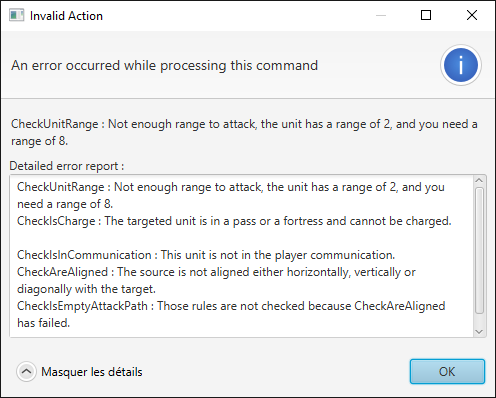
\includegraphics[width=0.7\textwidth]{interface/log}
\caption{Message d'erreur d'une commande d'attaque invalide}\label{fig:ui_log}
\end{figure}

\subsection*{Résultats d'affrontement}
Après une attaque, un message affichant le résultat de l'affrontement obtenu s'affiche, qu'il soit réussit ou non (voir figure \ref{fig:logAttack}).
\begin{figure}[!h]
\centering
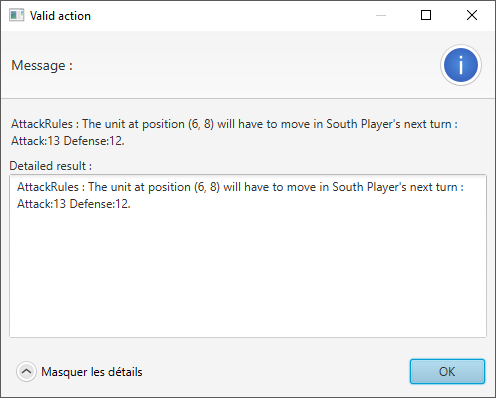
\includegraphics[width=0.7\textwidth]{interface/logAttack}
\caption{Message d'information à la suite d'une attaque}\label{fig:logAttack}
\end{figure}

\subsection*{Victoire}
Quand l'action d'un joueur mène à sa victoire, un simple message s'affiche pour l'en informer (voir figure \ref{fig:logVictory}).
\begin{figure}[!h]
\centering
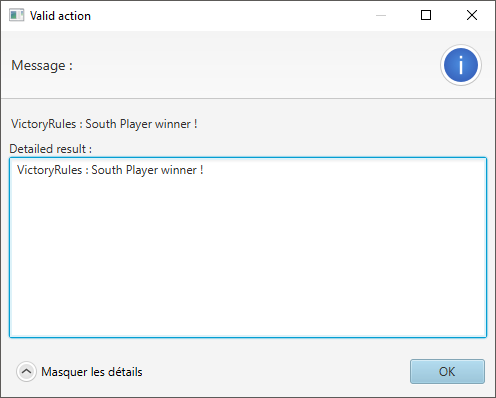
\includegraphics[width=0.7\textwidth]{interface/logVictory}
\caption{Message d'information à la suite d'une attaque}\label{fig:logVictory}
\end{figure}


%%%%%%%%%%%%%%%%%%%%%%%% ARCHITECTURE %%%%%%%%%%%%%%%%%%%%%%%%%%%%%%%%%%%%%%%%
\chapter{Architecture}

\section{Vue d'ensemble}

Lors de notre réflexion sur la structure générale du projet, nous avons très rapidement défini, avec notre chargé de TD, cinq modules principaux qui divisent les grandes lignes de notre projet. (voir \ref{fig:ex4modules})

\begin{enumerate}
\item Le moteur de règles, permettant de vérifier la validité d'un coup et de l'appliquer selon les règles décrites dans \textit{Jeu de la Guerre}.
\item L'état du jeu, qui stocke toutes les données nécessaire au déroulement de la partie et gère les accès au plateau.
\item Le moteur de jeu, qui est le cœur du programme. Il détient la boucle principale, et lie tous les autres modules entre eux. 
\item L'interface "joueur", qui représente un joueur réel ou artificiel.
\item Le module d'analyse, qui construit, à partir d'un état de jeu, des cartes d'informations diverses qui seront utiles autant pour un joueur réel que pour un système expert.

\end{enumerate}

%% L'architecture de notre projet se divise en quatre modules principaux, tout d'abord le module du joueur, comportant l'interface utilisateur et une représentation de celui-ci permettant de communiquer avec le jeu, puis le module représentant l'état du jeu, ensuite nous avons celui du moteur de règles qui est la représentation des règles décrites dans le \textit{Jeu de la Guerre} \cite{jdg}, et enfin la partie concernant le jeu, à savoir \textbf{Game}, qui permet de mettre en relation les modules précédents en fonction des entrées de l'utilisateur.

%% Afin de faciliter l'implémentation d'un système expert, un cinquième module a été ajouté, celui d'Analyse, qui vient se brancher directement au niveau de l'état du jeu et du moteur de règles afin de ne pas venir modifier le module du jeu. L'interface utilisateur se sert de ce module afin d'afficher une représentation graphique de ses calculs. Ce module, en plus de fournir des aides visuelles à l'utilisateur sur l'état de la partie, peut être utilisé par le système expert afin d'aider dans la réalisation de la stratégie définie, et donc dans l'application de tactiques.

Une documentation Javadoc est disponible concernant notre projet. Nous avons également utilisé l'outil Doxygen qui permet d'avoir, en plus de la génération de la documentation, une représentation plus visuelle de l'architecture et des dépendances entre les différents composants de notre projet.

\begin{figure}[!h]
\centering
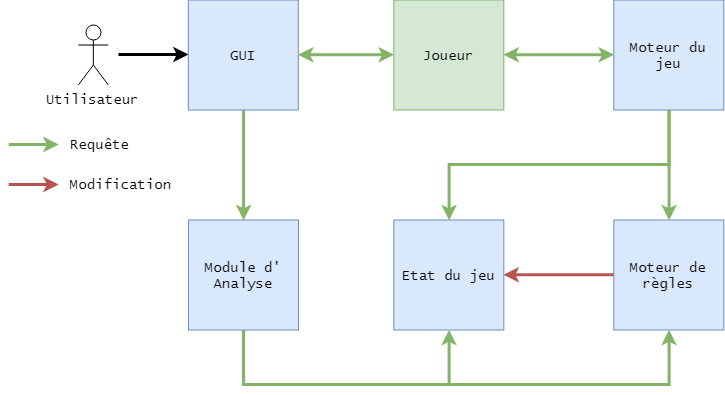
\includegraphics[width=0.85\textwidth]{UML/modules}
\caption{Interactions au sein de l'architecture du programme}\label{fig:ex4modules}
\end{figure}


\section{Moteur de règles} 
\label{sec:moteurDeRègles}
L'un des objectifs premiers lors de la conception du moteur de règles a été de le rendre le moins dépendant possible du reste du jeu. Le moteur de règles se divise en trois parties, \textbf{RuleChecker} qui s'occupe d'associer les actions à une des règles et de la tester, cette classe représente le point d'entrée du module utilisé par le jeu et par le module d'analyse. Nous avons aussi une classe représentant le résultat produit par la vérification des règles, à savoir le RuleResult qui sera transmis à l'issue d'une requête, et enfin la partie concernant les règles et leurs associations.

Pour faciliter la communication avec les autres modules, \textbf{RuleChecker} utilise une énumération, \textbf{EGameActionType}, qui représente chaque mécanisme décrit par le \textit{Jeu de la Guerre}.
La figure \ref{uml:UMLRuleChecker} représente un schéma UML des interactions entre le \textbf{RuleChecker} et les autre modules, ainsi que les classes du moteur de règles.

\begin{figure}[!h]
\centering
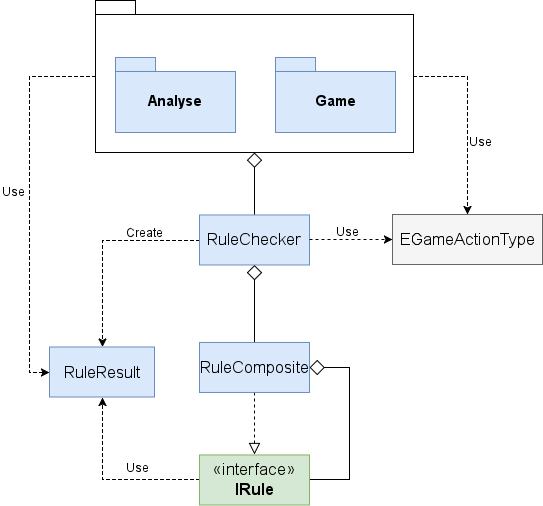
\includegraphics[width=1\textwidth]{UML/UMLRuleChecker.png}
\caption{Schéma UML du moteur de règles}\label{uml:UMLRuleChecker}
\end{figure}

Afin de conserver une certaine cohérence entre les sous-règles, un système de dépendances entre elles a dû être mis en place. Pour répondre à ce besoin, nous avons utilisé le patron de conception \textit{Composite} (voir figure \ref{uml:composite}). Le Composite nous permet d'avoir une structure d'arbre, où nous ne nous soucions pas de savoir si les règles partageant l'interface \textbf{IRule} sont des sous-règles, des règles ou des groupes de règles. \

Dans notre cas, ce patron nous permet de générer une structure d'arbre, où la partie composite du pattern, à savoir les nœuds, représente les opérateurs logiques \textit{ET}, \textit{OU} et \textit{NON}, et leurs équivalents paresseux servant de dépendances, et où les feuilles sont des sous-règles. Ainsi les règles, ou \textit{MasterRules}, étendent un des opérateurs logiques et spécialisent la méthode \path{applyResult()} afin d'appliquer au jeu les modifications associées à la règle. \label{archi:composite}

\begin{figure}[!h]
\centering
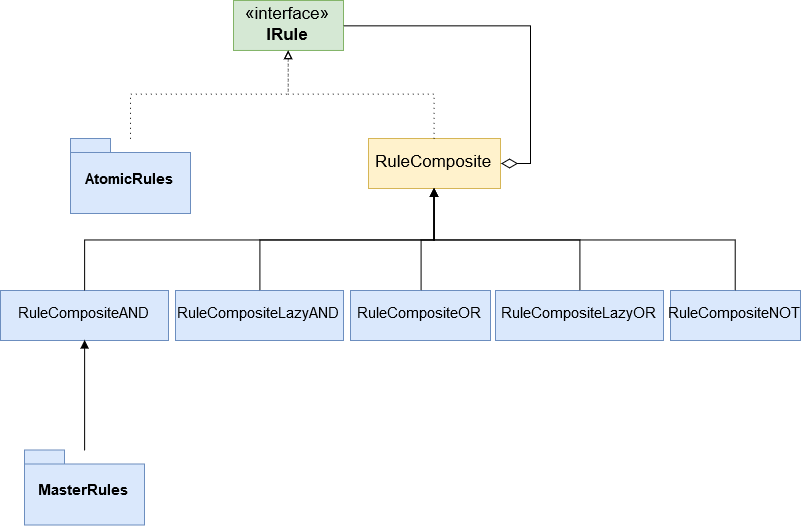
\includegraphics[width=1\textwidth]{UML/compositeRules.png}
\caption{Schéma UML des règles composites}\label{uml:composite}
\end{figure}

\section{\'Etat du jeu}

La classe \textbf{GameState} contient toutes les informations qui caractérisent une partie à un instant donné, et sert donc essentiellement de classe de stockage.
Elle contient un plateau, les listes des bâtiments et des unités ainsi que l'identifiant du joueur courant.

\begin{figure}[!h]
\centering
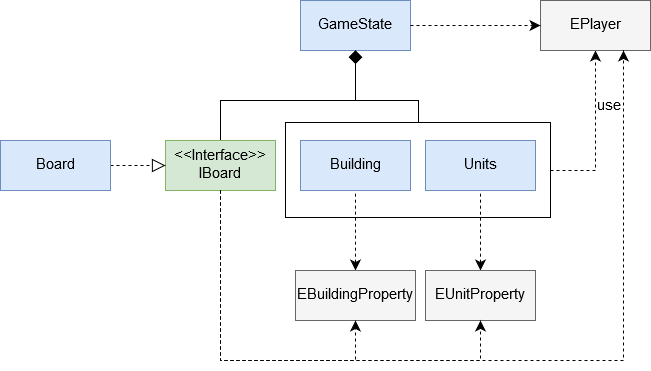
\includegraphics[width=1\textwidth]{UML/gameState.png}
\caption{Schéma UML de l'état du jeu}\label{uml:gameState}
\end{figure}

\section{Moteur de jeu}

Le moteur de jeu est la classe centrale du programme, qui relie les autres modules et les fait interagir entre eux. Il prend les commandes aux objets \textbf{Player}, donne le coup correspondant au moteur de règle avec le \textbf{GameState} à modifier, puis retourne la réponse au \textbf{Player}.

% Dans le cas où la commande n'est pas un coup à jouer, c'est un objet \textbf{UserToGameCall} qui
La commande est récupérée dans un \textbf{UIAction}, qui peut être interprété comme une commande pour agir sur le jeu ou bien effectuer une commande propre au programme, comme de la manipulation de fichier.
La réponse est elle envoyée sous la forme d'un \textbf{GameResponse}.

\begin{figure}[!h]
\centering
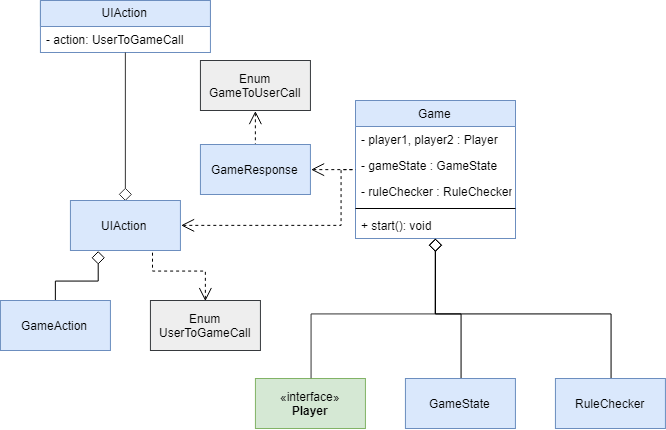
\includegraphics[width=1\textwidth]{UML/uml_game.png}
\caption{Schéma UML du moteur de jeu}\label{uml:game}
\end{figure}

\section{Interface utilisateur}

L'interface est centrée autour du la classe \textbf{TermGUI}, héritant de \textbf{Application} de JavaFX. Elle est composée de trois "Pane", un pour le panneau contenant les éléments de commandes, un autre les éléments d'informations et enfin un contenant les éléments du jeu.

Le schéma UML complet de ce module est relativement important (Voir figure \ref{uml:interface}), en partie car les éléments d'affichage sont séparés eux-même en plusieurs classes pour mieux diviser le code de l'interface.

C'est par le biais de \textbf{GUIPlayer}, implémentant \textbf{Player}, que l'interface enverra les commandes et recevra les réponses du jeu.
\begin{figure}[!h]
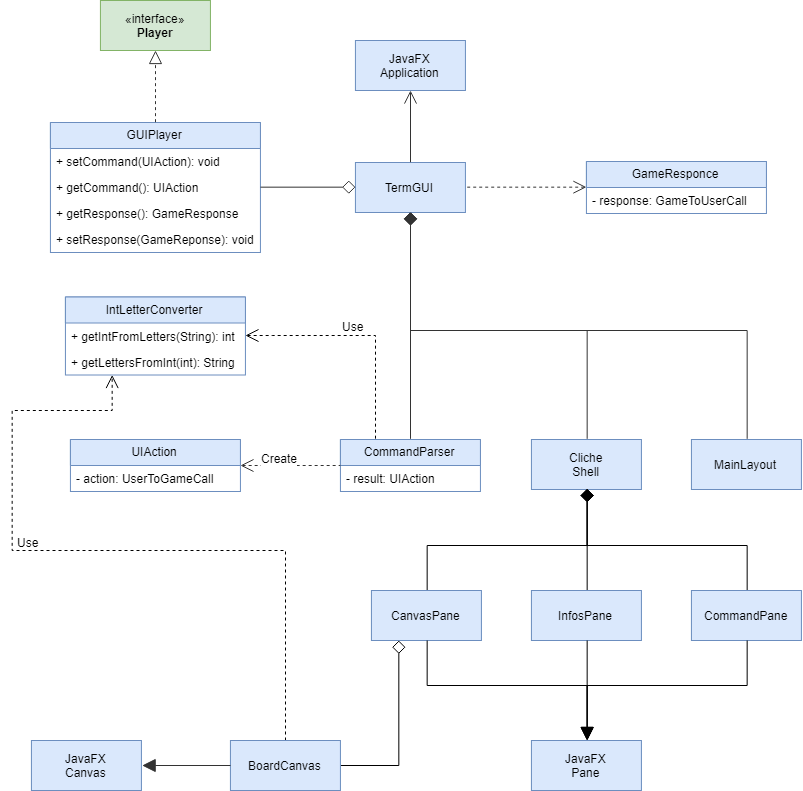
\includegraphics[width=1\textwidth]{UML/uml_interface.png}
\caption{Schéma UML de l'interface utilisateur}\label{uml:interface}
\centering
\end{figure}

\section{Module d'analyse}

Le module d'analyse n'étant pas essentiel au déroulement d'une partie, celui-ci se doit de ne pas servir de dépendance aux autres modules, tout en restant accessible au niveau d'un objet implémentant l'interface \textbf{Player}, afin qu'une interface graphique ou bien un joueur artificiel puisse l'exploiter.

Le point d'entrée de ce module se fait par la classe \textbf{InfoModule} via des méthodes publiques et statiques, pour obtenir une architecture "annexe" de ce que nous avons déjà produit.

Chaque algorithme d'analyse implémente une interface définissant le type informatique de la donnée retournée (actuellement, \textbf{IMetricMapType} et \textbf{IMetricMoveType} retournent respectivement un tableau en deux dimensions de \texttt{double} et une liste de mouvements). \textbf{InfoModule} s'adapte à ces interfaces et sert de passerelle pour accéder à ces informations.
Les algorithmes sont ensuite répertoriés dans des énumérations, ces dernières possédant des références vers ces dits algorithmes. Une requête au module d'analyse se fait donc en appelant \textbf{InfoModule} et en indiquant l'information désirée à l'aide de ces énumérations.


\begin{figure}[!h]
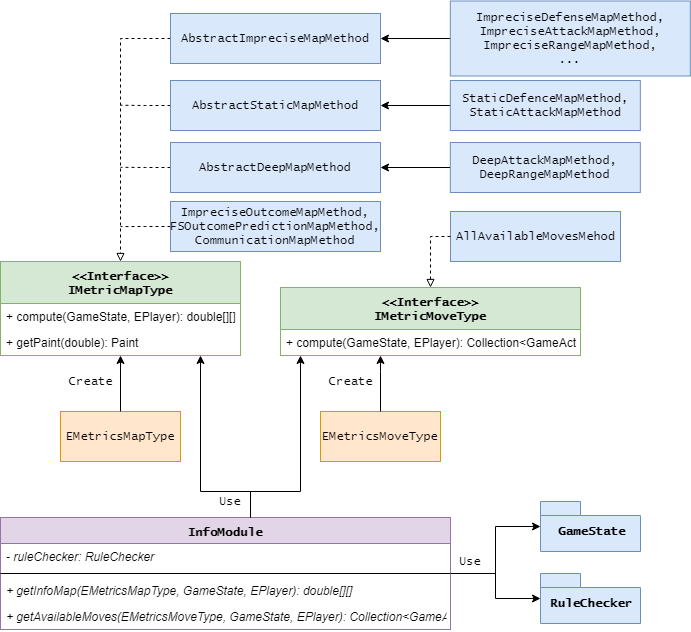
\includegraphics[width=1\textwidth]{UML/umlAnalyse.png}
\caption{Schéma UML du module d'analyse}\label{uml:analyse}
\centering
\end{figure}

%%%%%%%%%%%%%%%%%%%%%% IMPLEMENTATION %%%%%%%%%%%%%%%%%%%%%%%%%%%%%%%%%%%%%%%%%%%%%%%
\chapter{Implémentation}
\section{Modules principaux}

Si, lors du développement, nous avons changé un certain nombre des décisions prises plus tôt dans le projet, les modules ont très peu été altérés jusqu’à la fin du développement, et représentent la base sur laquelle nous avons imaginé et créé nos classes pour tout le programme.

Dans les sections suivantes, nous détaillons le fonctionnement et l'implémentation de ces modules.	

\section{Moteur de jeu}

\subsection{Jeu (Classe Game)}

La classe \textbf{Game} comprend deux joueurs, un état de jeu (dont le plateau), et le moteur de règles. 

Son but est de faire communiquer ses différents membres entre eux pour s'assurer du bon déroulement du jeu.

\begin{figure}[H]
\centering
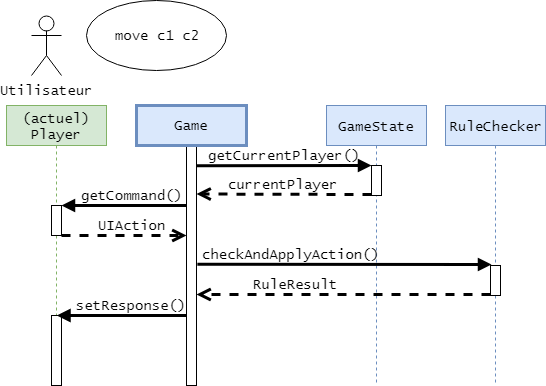
\includegraphics[width=0.8\textwidth]{sequences/game.png}
\caption{Diagramme de séquence du Jeu}\label{seq:game}
\end{figure}

Dans un premier temps, \textbf{Game} demande une commande au joueur dont c'est le tour, la donne au moteur de règles pour la vérifier et l'appliquer si elle est correcte, puis retourne la réponse et le nouvel état du plateau au joueur. Deux types de commandes sont différenciés : les commandes de jeu (\texttt{move} et \texttt{attack}), qui seront transmises au moteur de règles, et les commandes \texttt{save}, \texttt{load} et \texttt{revert} qui sont gérées au sein de cette classe.

L'historique des états de jeu est également stocké dans cette classe, lorsqu'une modification se produit sur l'état actuel du jeu, sous la forme d'une pile de \textbf{GameState} dont nous pouvons dépiler la tête lorsque l'utilisateur appelle la commande {\tt revert}.

Nous nous sommes efforcés de garder cette classe aussi réduite que possible, afin d'éviter de lui donner trop de responsabilités, car sa situation centrale lui donne beaucoup de pouvoir sur les objets qui la composent. 

\subsection{Plateau de jeu (Classe Board)}

Nous aurions pu représenter le plateau sous la forme de listes d'objets et de coordonnées, mais cela aurait rendu sa manipulation (tel que savoir si une unité peut se déplacer sur une case) et surtout l'analyse (tel que le calcul et l'affichage des communications), beaucoup plus difficile. Nous avons néanmoins rapidement pris en compte le fait que l'implémentation d'un module d'analyse pourrait avoir besoin de nombreuses copies du plateau en différents états, aussi l'occupation mémoire et le temps de clonage a été un point crucial lors de sa conception.

Nous avons donc rapidement abandonné la représentation sous la forme d'un tableau d'objets cellules contenant des informations, car trop coûteux, pour une représentation par tableaux de primitives, manipulés à l'aide d'opérations sur les bits.

Le plateau est représenté par deux tableaux de \texttt{short} (unités et bâtiments) et un tableau de \texttt{byte} pour représenter les communications, chacun de taille $hauteur*largeur$ \ref{fig:board_bits}.

\begin{figure}[h]
\centering
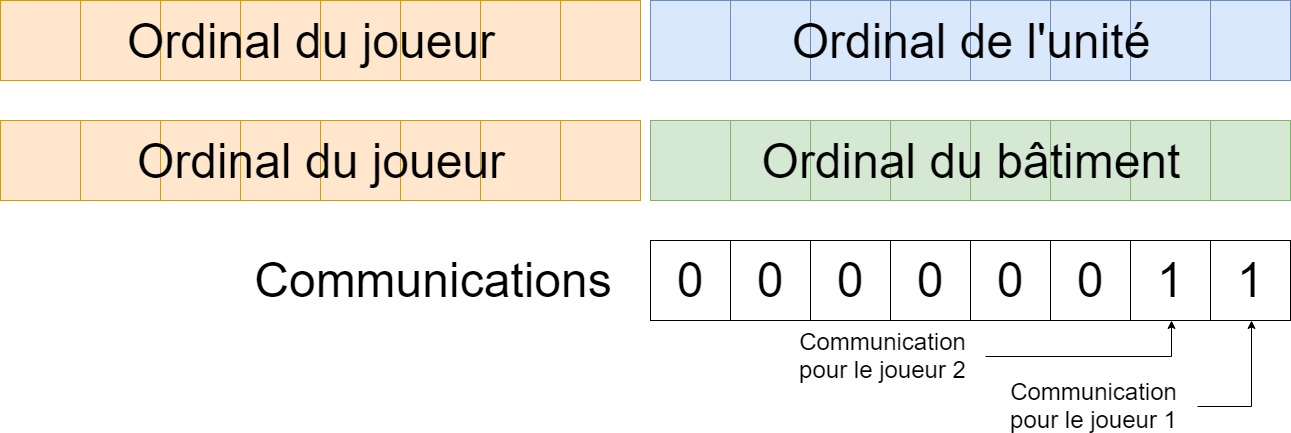
\includegraphics[width=0.5\textwidth]{implementation_game/pdp_board_bits}
\caption{Contenu des primitives de \texttt{Board}}
\label{fig:board_bits}
\end{figure}

Cela nous donne, pour le plateau de \textit{Jeu de la Guerre} de taille $25*20$, deux tableaux de 500 \texttt{short} et un tableau de 500 \texttt{byte}, ce qui demande donc $2*500*(2 octets) + 500*(1 octet) = 2.5Ko$ pour représenter le plateau.

Un certain nombre de méthodes privées dédiées à abstraire les manipulations bit à bit ont été créées pour réduire au maximum la nécessité de les manipuler au sein même de la classe :
\begin{itemize}
\item \texttt{getOffset()} sert à atteindre la case correspondantes aux coordonnées [x,y] dans des tableaux à une dimension.
\item \texttt{getUnitType()}, \texttt{getBuildingType()} et \texttt{setItemType()} permettent d'atteindre la partie de l'octet correspondant au type des bâtiments ou unités de la case.
\item \texttt{getPlayer()}, \texttt{setItemPlayer()} permettent d'atteindre le joueur propriétaire.
\end{itemize}

Les autres méthodes, à part pour les communications, n'ont donc pas à manipuler les primitives mais peuvent utiliser directement les énumérations des joueurs, unités et bâtiments en composant les appels de ces méthodes privées.

Les méthodes sont faites pour être appelées sur des cases valides (par exemple {\tt getUnitPlayer()} doit être appelée pour une case avec une unité), et lèvent l'exception personnalisée \texttt{IllegalBoardCallException} si ce n'est pas le cas.

Étant donné que \texttt{Board} fournit les méthodes pour s'assurer qu'un appel est valide (tel que {\tt isUnit()} pour le cas précédent), cette exception hérite de \texttt{RuntimeException} et n'est donc pas nécessairement testée par les appelants.

Nous avons également ajouté un tableau et les accesseurs associés pour effectuer un marquage sur les cases, qui est notamment utilisé pour le calcul des communications et peut être utilisé pour le module d'analyse.
Également, la méthode \texttt{clone()} du plateau, massivement utilisée par ce module, utilise le fait que Java puisse copier très efficacement les tableaux de primitives en natif.

\subsection{\'Etat du jeu (Classe GameState)}

La classe GameState a été créée afin de représenter l'état du jeu à un moment donné, et sera par exemple utilisée, en plus du jeu, par le moteur de règles et le module d'analyse, ainsi que pour la commande revert.

Cette classe comprend une représentation du plateau, et des informations complémentaires comme le tour du joueur actuel, le nombre de coups restant, la liste des unités de chaque joueur et quelques autres informations nécessaires au moteur de règles. Nous avons choisi de créer ces listes afin d'avoir accès sans itérer sur le plateau aux unités et aux bâtiments.

Une liste des unités battant en retraite à dû être ajoutée à cela afin d'être communiquée au moteur de règle.

Le plateau est totalement abstrait par cette classe, afin que seule cette classe puisse le modifier, elle comprend donc un grand nombre de méthodes "wrapper" qui se contentent de passer des appels au Board.


\begin{figure}[!h]
\centering
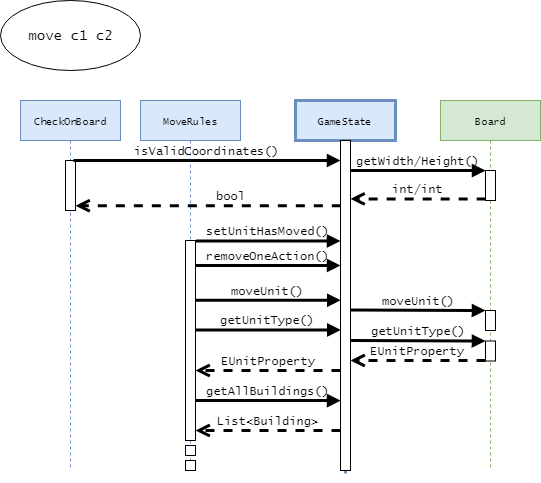
\includegraphics[width=0.9\textwidth]{sequences/sequenceGameState.png}
\caption{Diagramme de séquence du GameState}\label{seq:gamestate}
\end{figure}

\subsection{Joueur (Interface Player)}
Les joueurs sont les objets auxquels la classe Game s'adresse directement pour obtenir les commandes à jouer. Ils jouent le rôle d'interface entre le joueur "réel" (humain ou machine) et le jeu.

Afin de renforcer l'indépendance entre Game et les Player, les classes de joueurs implémentent l'interface Player qui se résume à quatre méthodes : {\tt get/setCommand()} et {\tt get/setResponse()}.
Ainsi, le jeu pourra appeler le {\tt getCommand()} du joueur actuel, et après avoir traité la commande donnera sa réponse par {\tt setResponse()}.

En parallèle, la classe qui est chargée de donner les commandes (GUI par exemple), appellera {\tt setCommand()} puis {\tt getResponse()}.

Bien entendu, les appels n'étant pas synchrones, la classe Player se charge donc de la synchronisation, de telle sorte qu'elle soit invisible pour les threads appelant : les commandes {\tt get()} sont bloquantes et retournent toujours le résultat attendu dès qu'il est disponible \ref{fig:player_synchro}.
\begin{figure}[h]
\centering
\rotatebox{90}{
	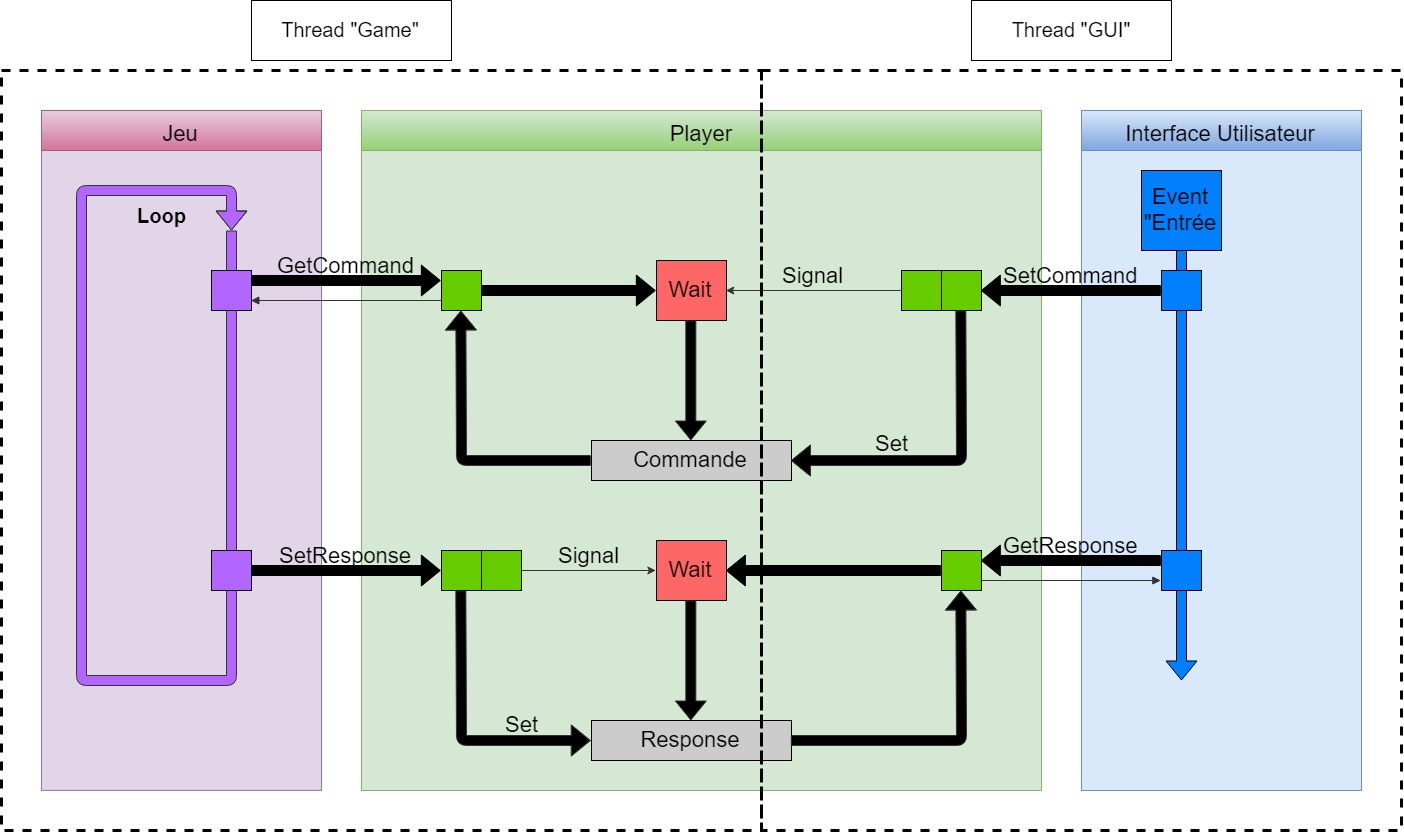
\includegraphics[width=1.5\textwidth]{implementation_game/player_synchro}
}
\caption{Schéma de la synchronisation entre le Jeu (Game) et l'interface utilisateur}
\label{fig:player_synchro}
\end{figure}

Nous avons deux implémentations de joueurs : 

La première est GUIPlayer, qui représente un joueur "Humain" qui communique via l'interface. La construction de la classe rend la nature asynchrone de l'interface JavaFX très facile à gérer, il suffit d'appeler {\tt setCommand()} lorsque la commande est rentrée par l'utilisateur.

La seconde implémentation est le BotPlayer, qui est une ébauche de système expert destinée à déterminer des coups à jouer. Dans sa forme actuelle, les commandes sont générées à l'appel de {\tt getCommand()}. Il faudrait à terme avoir un thread séparé qui les génère de manière asynchrone, mais cela nécessiterait quelques modifications que nous n'avons pas eu le temps d’apporter.

\section{Moteur de règles}

Comme décrit dans la partie \ref{sec:moteurDeRègles}, le moteur de règles est un point essentiel du projet, et son implémentation a évolué de nombreuses fois, notamment pour développer le système de dépendances que nous décrirons plus tard.

L'objectif principal que nous avions était d'avoir un moteur de règles permettant de modifier le contenu de ces règles sans modifier le code du moteur.

Lors de la retranscription informatique des règles, nous nous sommes rendu compte de duplication de vérification, et donc de code. Afin de conserver l'atomicité des sous-règles, et permettre de générer des messages de refus exhaustifs sans générer de problème lors de la vérification, nous avons dû mettre en place un système de dépendances. 
Par exemple, nous voulions vérifier une seule fois si les coordonnées entrées par l'utilisateur représentaient bien une case présente sur le plateau, afin d'éviter aux autres sous-règles demandant des accès au plateau de les vérifier à nouveau.

Dans un premier temps, ces dépendances étaient gérées par les master-rules via un système de {\it Map}, qui, à chaque règle vérifiée, attribuait en valeur le résultat de cette règle. Ces résultats étaient vérifiés à chaque fois qu'une sous-règle était appelée, mais cette méthode s'est avérée difficilement maintenable.
Ce système de dépendance a donc été ré-implémenté sous la forme d'un arbre, parcouru par les master-rules suivant la nature des nœuds de l'arbre, pouvant être des règles, ou bien des opérateurs logiques {\it ET}, {\it OU}, ou {\it NON}, avec leurs équivalents paresseux. Ces arbres sont décrits dans la section \ref{sssec:composites}. %section arbres logiques

Notre moteur de règles est défini par trois modules, le RuleChecker, qui communique avec le Game via le RuleResult, collectant les messages générés par les règles sur une action et stocke la validité de celle-ci, et les règles qui sont définies en trois parties, les sous-règles qui ont une unique responsabilité, les règles qui sont la représentation des actions décrites dans le livre, et les composites logiques, qui servent de liant entre les règles et les sous-règles.

\subsection{Vérificateur de règles (Classe RuleChecker)}

La classe RuleChecker est la classe communiquant avec le jeu (Game), elle représente le point d'entrée du moteur de règles et permet donc de vérifier la règle associée à l'action proposée par celui-ci sur une instance du plateau. Avant de commencer la vérification de la règle, elle crée un RuleResult qu'elle donnera à celle-ci afin de récupérer les messages et la validité de l'action avant de les renvoyer au jeu.

Cette classe fournit deux services, la simulation d'une action à l'aide de la méthode {\tt checkAction()}, et la vérification suivie de l'application de la règle à l'aide de la méthode {\tt checkAndApplyAction()}. Lors du déroulement d'une partie, la méthode {\tt checkAndApplyAction()} est celle utilisée pour traiter une entrée provenant d'un joueur. En effet, la simulation sert principalement au joueur automatique à travers le module d'analyse.

\begin{figure}[!h]
\centering
\rotatebox{90}{
	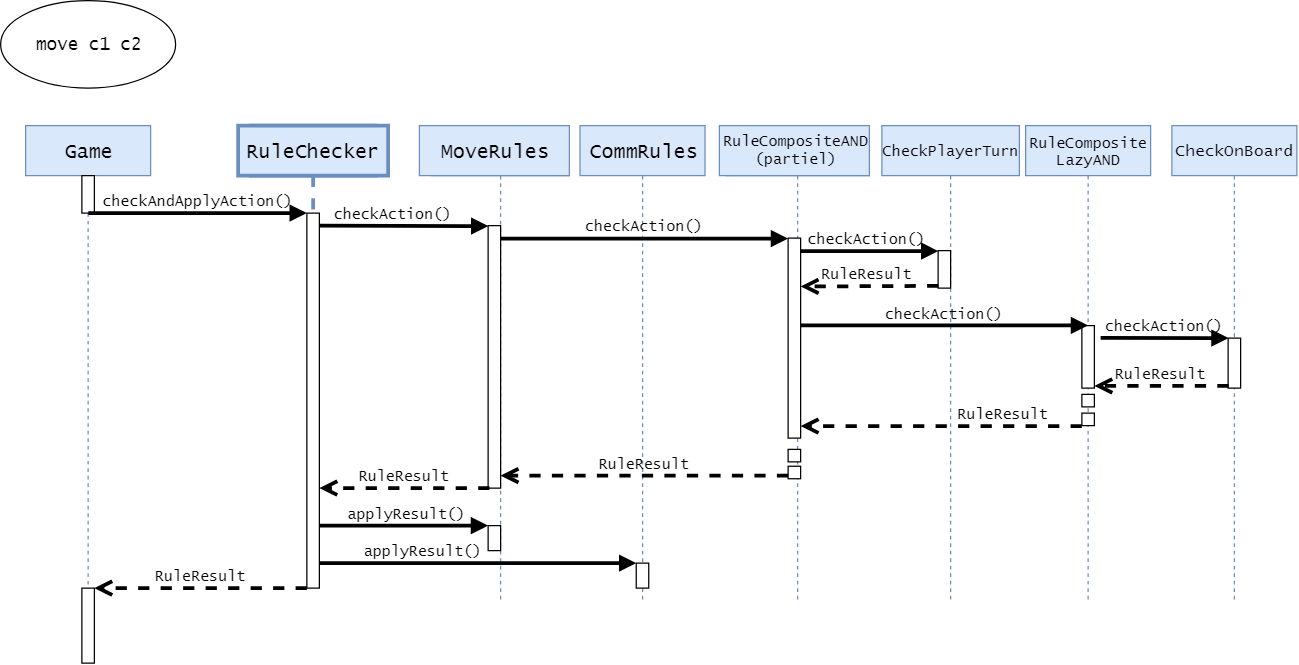
\includegraphics[width=1.5\textwidth]{sequences/sequenceRuleChecker.png}
}
\caption{Diagramme de séquence du RuleChecker}\label{seq:ruleChecker}
\end{figure}

\subsection{Résultat d'une vérification (Classe RuleResult)}

La classe RuleResult permet de recueillir les messages produits par les règles ainsi que la validité de l'action proposée. La validité de l'action est initialisée à vrai lors de la création du RuleResult, et peut être invalidée par les règles lors de la vérification, cependant elle ne pourra plus être remise à valide.

Ces messages sont en lien direct avec le besoin concernant la génération de messages expliquant le refus de l'action proposée, ils sont générés par les sous-règles qui explicitent ce qui n'allait pas avec la proposition de l'utilisateur en fonction de l'état du jeu actuel.

\subsection{Gestion des règles}
\subsubsection{Les sous-règles}
Les sous-règles sont décrites comme des règles "atomiques" car on leur attribue une unique responsabilité, une seule vérification, la plus fine possible. Elles implémentent l'interface IRule et n'utilisent que la méthode {\tt checkAction()}, qui prend une instance du plateau et un RuleResult, afin d'invalider ou non le résultat et d'y ajouter un message correspondant à l'invalidation de l'action.

Par exemple, la règle CheckIsAllyUnit va vérifier si les coordonnées sources contenues dans le GameAction pointent bien vers une unité alliée sur le plateau, sinon, la règle va ajouter un message expliquant le problème (si c'est une unité ennemie ou si tout simplement il n'y a pas d'unité sur cette case) et invalider le résultat. 


\subsubsection{Les règles composites logiques}\label{sssec:composites}

Ce type de règles nous permet d'utiliser 5 opérateurs logiques, le ET et le OU, leurs équivalents paresseux, et le NON. Elles spécialisent toutes la méthode {\tt checkAction()} afin de correspondre à l'opérateur logique associé, ainsi les règles composant l'un de ces opérateurs logiques seront vérifiées et modifieront le résultat si les règles satisfont l'opérateur en question.

Pour gérer les dépendances, les opérateurs paresseux ET et OU sont utilisés. Le ET paresseux vérifie les règles dans l'ordre, et lorsqu'une règle échoue, il arrête d'appeler la méthode {\tt checkAction()} des autres règles et génère un message expliquant que les règles suivant celle qui a échoué en sont dépendantes, et donc n'ont pas été vérifiées. Le OU paresseux fonctionne de la même manière, à la différence qu'il s'arrête de vérifier les règles dès qu'une est valide.

Les classes associées aux opérateurs ET, ET paresseux, OU, OU paresseux et NON sont respectivement RuleCompositeAND, RuleCompositeLazyAND, RuleCompositeOR, RuleCompositeLazyOR et RuleCompositeNOT. Elles étendent toutes la classe abstraite AbsRuleComposite qui implémente l'interface IRule et qui contient une liste chaînée de règles IRule, cette liste servira à la vérification des règles lors de l'appel à {\tt checkAction()}.

\begin{figure}[!h]

\begin{minipage}{.5\textwidth}
\centering

%\centering
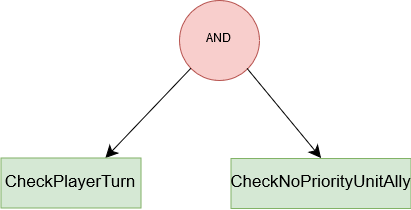
\includegraphics[width=0.8\textwidth]{treeRules/ArbreEndRules.png}
\caption{Arbre des règles de fin de tour}
\label{fig:treeEnd}

\end{minipage}
\hfill
\begin{minipage}{.5\textwidth}
\centering

%\centering
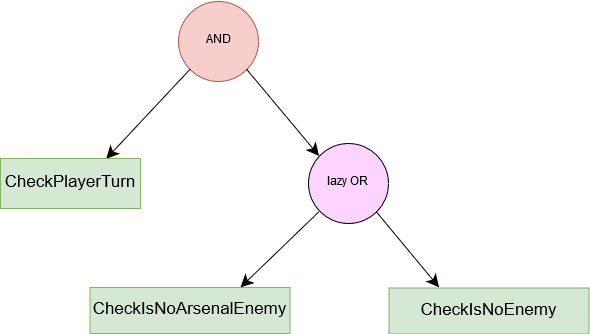
\includegraphics[width=1\textwidth]{treeRules/ArbreVictoryRules.png}
\caption{Arbre des règles de victoire}
\label{fig:treeVictory}

\end{minipage}

\end{figure}

\subsubsection{Les règles (MasterRule)}

Les règles mères sont associées à un mécanisme explicite, comme le déplacement décrit dans le livre, ou implicite, comme les conditions pour passer son tour. Elles étendent l'une des règles composites logiques afin de définir l'ordre des vérifications et les dépendances entre les règles qui la composent.

La composition logique des sous-règles se fait dans le constructeur de la règle mère, c'est ici que l'on crée et assemble les groupes de règles en leur associant un opérateur logique.

Ainsi nous avons 5 règles mères différentes, la règle de déplacement MoveRules \ref{fig:treeMove}, la règle d'attaque AttackRules \ref{fig:treeAttack}, la règle de fin de tour EndRules \ref{fig:treeEnd}, la règle de victoire VictoryRules \ref{fig:treeVictory} et la règle de communication CommRules. Chacune peut être représentée par un arbre grâce au patron de conception Composite (voir \ref{archi:composite}), l'ordre de vérification effectué lors de l'appel à {\tt checkAction()} correspond à l'ordre préfixe des arbres.

Ces règles doivent spécialiser la méthode {\tt applyResult()} afin d'apporter les modifications associées à elles à l'état du jeu passé en paramètre.

Afin d'afficher dans la console une représentation textuelle des arbres, la méthode \texttt{getName()} permet aux classes composites de retourner une chaîne de caractère qui est composée du nom des règles qui les composent ainsi que des opérateurs logiques qui les lient.

La règle de communication étant un comportement spécifique au jeu mais ne dépendant d'aucune règle, donc n'en vérifiant aucune, elle permet simplement de recalculer les communications sur l'état du jeu tel qu'il est défini dans le livre lors de l'appel à la méthode {\tt applyResult()}.

\paragraph*{Calcul des communications}\label{calculComs}

\paragraph*{}

Le calcul des communications est le mécanisme le plus important du \textit{Jeu de la Guerre}, toutes les actions de déplacement, d'attaque et de défense en sont dépendantes. 

Notre implémentation du calcul des communications est une fonction récursive, qui propage la communication depuis une case dans une direction, avec une limite de portée, -1 si infinie. La communication étant créée et diffusée par les arsenaux, nous exécutons cette fonction récursive dans les 8 directions pour chaque arsenal présent sur le plateau.

Cette fonction récursive s'arrête lorsqu'elle se trouve sur une case hors du plateau, sur une montagne, sur une unité ennemie combattante ou si nous avons atteint la limite de portée définie par l'arsenal ou unité à l'origine de cette communication. Nous ignorons les cases contenant des unités alliées déjà visitées. La récursivité de cette fonction doit s'arrêter grâce aux coordonnées qui évoluent dans une seule direction, ainsi à un moment nous atteindrons forcément l'un des bords du plateau, et aussi du fait que nous ne considérons plus les unités déjà traitées, ces conditions permettant l'arrêt la fonction.

\newpage
La complexité de notre implémentation (voir algorithme \ref{alg:communication}) peut s'écrire sous la forme 
$$
O((nbRelay + nbArsenal) * (3 * min(H, W) + max(H, W)) + nbUnits * 8)
$$
où chaque symbole représente :
\begin{itemize}
\item $nbRelay$ le nombre d'unités relais,
\item $nbArsenal$ le nombre d'arsenaux,
\item $H$ la hauteur du plateau,
\item $W$ la largeur du plateau,
\item $nbUnits$ le nombre d'unités combattantes.
\end{itemize}

%%%%%%%% BEGIN PSEUDO CODE

\begin{algorithm}
\caption{Calcul des lignes de communication}\label{alg:communication}
\begin{algorithmic}[1]

\Procedure{computeCommunication}{$gameState$}\Comment{Fonction entrante}
\State \Call{clearCommunication}{$gameState$}
\State \Call{clearMarked}{$gameState$}\Comment{On remet à zéro le marquage du plateau}
\ForAll{$arsenal \in gameState$}
	%\State $x\gets \Call{getX}{arsenal}$
    %\State $y\gets \Call{getY}{arsenal}$
    \State $coordinates\gets$ \Call{getCoordinates}{$arsenal$}
    \State $player\gets$ \Call{getPlayer}{$arsenal$}
    %\State \Call{setInCommunication}{$gameState, player, x, y, true$}
    \State \Call{setInCommunication}{$gameState, player, coordinates, true$}
    \State \Call{setMarked}{$gameState, coordinates, true$}
    \ForAll{$d \in Directions$}\Comment{Dans les 8 directions}
    	\State \Call{createCom}{$gameState, coordinates, d, player, -1$}
    \EndFor
\EndFor
\EndProcedure
\Statex
\Procedure{createCom}{$gameState, coordinates, direction, player, rangeMax$}
    \State $coordinates\gets coordinates + direction$ 
    \State $distance\gets 1$
    \While{\Call{canContinue}{$gameState, coordinates, player, distance, rangeMax$}}
    	\State \Call{setInCommunication}{$gameState, player, coordinates, true$}
        \If{\Call{isAllyUnitUnmarked}{$gameState, coordinates, player$}}
        	\State \Call{setMarked}{$gameState, player, coordinates, true$}
            \State $range\gets 1$
            \If{\Call{isRelayUnit}{$gameState, coordinates$}}
            	\State $range\gets -1$
            \EndIf
            \ForAll{$d \in Directions$}
            	\State \Call{createCom}{$gameState, coordinates, d, player, range$}
            \EndFor
        \EndIf
        \State $coordinates\gets coordinates + direction$ 
        %\State $x\gets x + direction.X$
        %\State $y\gets y + direction.Y$
    \EndWhile
\EndProcedure
\Statex
\Function{canContinue}{$gameState, coordinates, player, distance, rangeMax$}
	%!isObstacle(gameState, x, y, player) && (rangeMax < 0 || dist <= rangeMax)
    \State $canContinue\gets $\Call{isNotFightingEnemyUnit}{$gameState, coordinates, player$}
	\State $canContinue\gets canContinue$ $\wedge$  \Call{isNotMountain}{$gameState, coordinates$}
    \State $canContinue\gets canContinue \wedge (rangeMax < 0 \vee rangeMax \ge distance)$
    \State \textbf{return} $canContinue$
\EndFunction

\end{algorithmic}
\end{algorithm}

\begin{figure}[h]
\centering
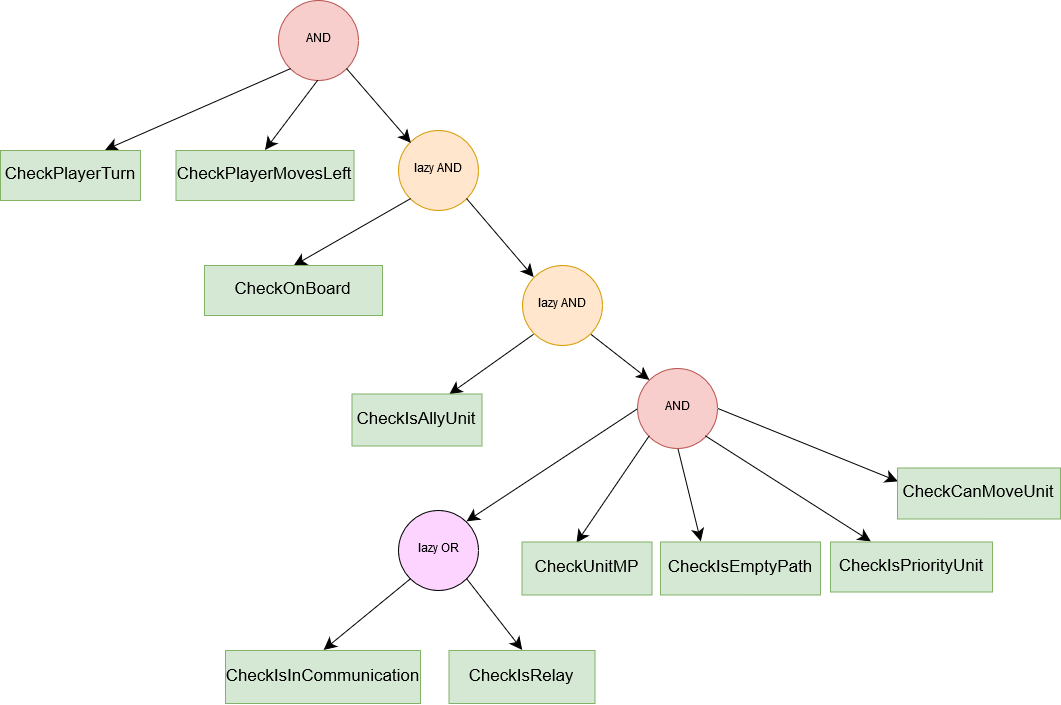
\includegraphics[width=1\textwidth]{treeRules/ArbreMoveRules.png}
\caption{Arbre des règles de déplacement}
\label{fig:treeMove}
\end{figure}

\begin{figure}[h]
\centering
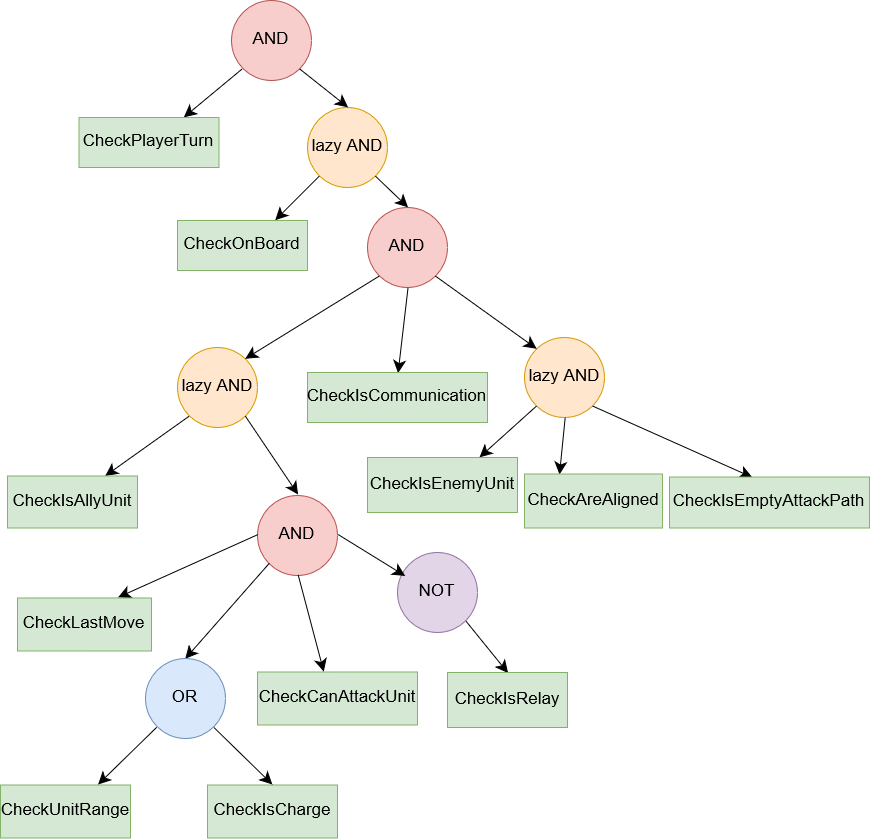
\includegraphics[width=0.8\textwidth]{treeRules/ArbreAttackRules.png}
\caption{Arbre des règles d'attaque}
\label{fig:treeAttack}
\end{figure}


\section{Interface utilisateur (Paquetage UI)}

L'interface utilisateur est un élément qui a beaucoup évolué au long du développement du projet. Nous avons commencé par un affichage simple du plateau dans une fenêtre JavaFX et les commandes étaient envoyées par le terminal. Pour l'analyse syntaxique, nous avons utilisé la bibliothèque Cliche \cite{cliche}, qui nous permet très facilement de traduire du texte vers des appels de méthode. La classe CommandParser endosse ce rôle, à travers des méthodes comme {\tt move(src, dst)}, appelées par Cliche lorsqu'on lui donne une chaîne de caractères "move [SRC] [DST]". Les coordonnées données sont au format lettres+chiffres comme précisé dans le cahier des besoins, et les lettres sont donc traduites de la base 26 vers la base 10 avant d'être utilisées.

Nous avons rapidement déplacé les commandes du terminal vers un champ de texte sur l'interface pour en simplifier l'utilisation, puis avons amélioré l'affichage avec des icônes, une légende, et enfin un menu pour choisir quel type de données afficher en fond sur le plateau.

La classe principale de l'interface est TermGUI (NOM A CHANGER ?), héritant d'Application de JavaFX. Les différents éléments d'interface sont ensuite factorisés en plusieurs classes pour éviter de déclarer tous les éléments à la suite dans une seule méthode. La plupart sont donc déclarées comme héritant d'une classe JavaFX, comportent très peu de code, et sont liées entre elles afin de respecter les changements de la taille de la fenêtre.

Le BoardCanvas, lui, est relativement chargé, c'est lui qui s'occupe d'afficher le plateau à l'aide de méthodes de dessin sur canvas. Afin de ne pas surcharger la classe avec beaucoup d'appels de dessin, une partie est déportée vers des méthodes statiques de la classe BoardDrawer qui se charge par exemple d'afficher les icônes. (voir \ref{fig:plateau}).

\begin{figure}[h]
\centering
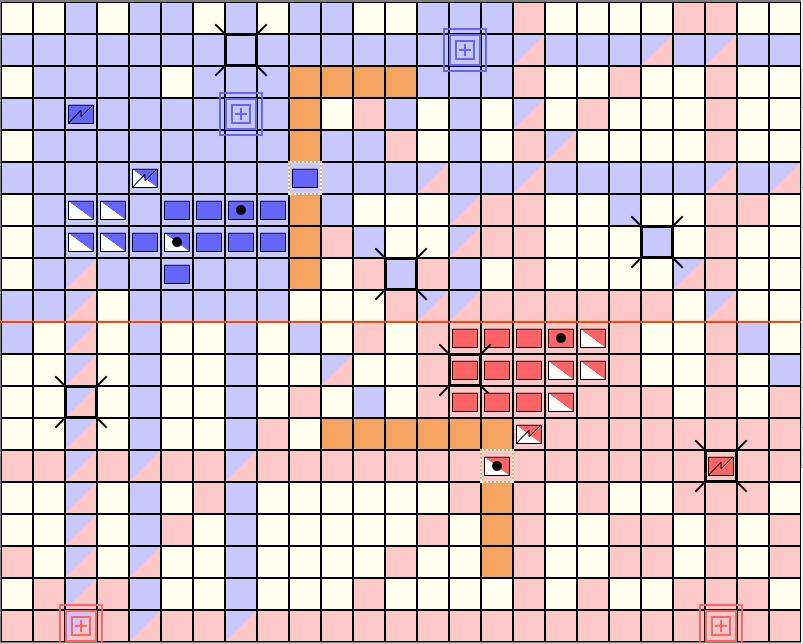
\includegraphics[width=0.8\textwidth]{interface/plateau}
\caption{Représentation du plateau}\label{fig:plateau}
\end{figure}

L'interface répond uniquement aux événements d'entrée et ne rafraîchit l'affichage que lorsque le plateau ou la fenêtre ont changé pour ne pas utiliser inutilement des ressources.

De même, afin de ne pas briser l'idée de segmentation de base du projet (avec les quatre modules), l'interface communique uniquement avec les objets Player à l'aide successivement de {\tt setCommand()} puis de {\tt getResponse()} lorsque l'utilisateur envoie une commande. Si la réponse fait écho à une commande invalide ou une fin de partie, cette information est affichée par une fenêtre 'pop-up'.

L'interface graphique fait néanmoins appel aux méthodes statiques du module d'analyse pour calculer les valeurs à afficher selon le type d'information demandé par l'utilisateur (voir \ref{fig:ui_full_attack}).

\begin{figure}[h]
\centering
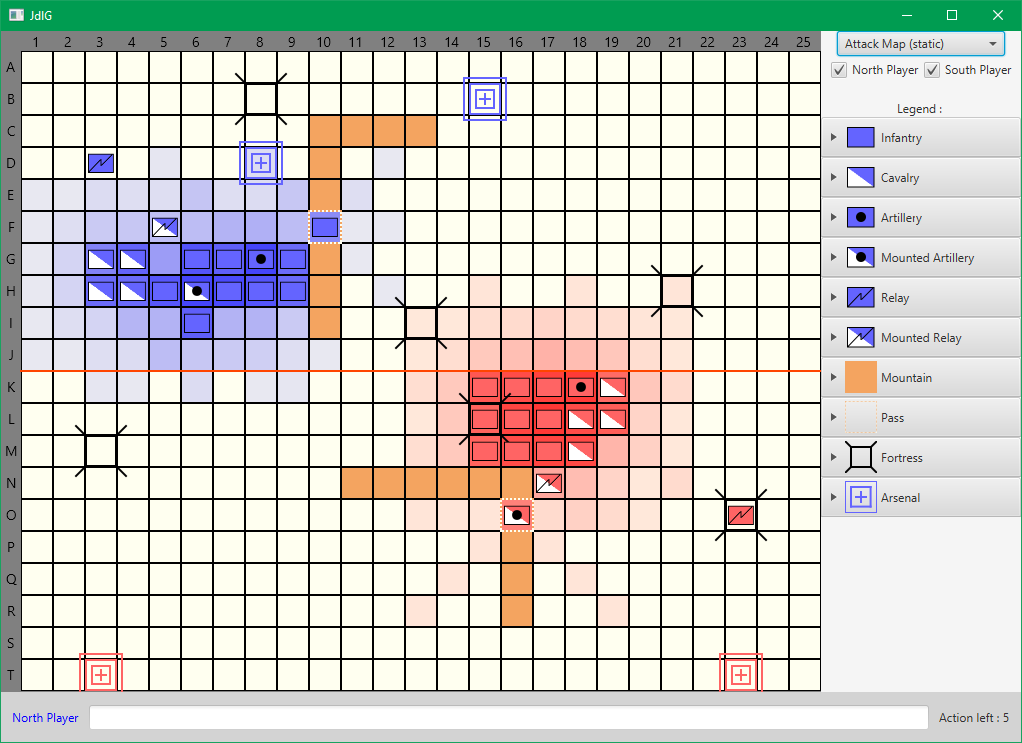
\includegraphics[width=1.0\textwidth]{interface/ui_full_attack}
\caption{Affichage de la carte d'attaque}\label{fig:ui_full_attack}
\end{figure}

\section{Module d'analyse}
\label{sec:analyse}
\subsection{Présentation}
Le module d'analyse a été implémenté de façon à n'avoir aucun impact sur le déroulement du programme, et peut donc fournir des informations relatives à la partie sur demande d'un objet client, comme un joueur voulant bénéficier d'une aide visuelle ou un joueur automatique lors d'une prise de décision. Le module d'analyse permet actuellement de générer des cartes d'informations, mais aussi de générer une liste de coups en suivant des directives.

Des algorithmes d'analyse simples ont été implémentés, sans se soucier de leur complexité, pour montrer de quoi était capable le programme.
Ces algorithmes sont le calcul des potentiels d'attaque, de défense, de portée et de prédiction de résultats d'affrontement. Les résultats de ces calculs peuvent être visualisés sur le GUI sous forme de cartes à nuances de couleurs. Une liste exhaustive de mouvements valides peut aussi être générée, et est utilisée par le joueur automatique implémenté.

Les algorithmes de potentiels d'attaque et de défense utilisent :
\begin{itemize}
\item L'état statique du plateau, sans considérer de mouvements. C'est la méthode utilisée dans le programme développé par le groupe de PdP 2014, et est utile surtout pour calculer les portées de défense des unités (adverses ou alliées), vu qu'une attaque demande un déplacement préalable de l'unité attaquante.
\item L'état du plateau après le déplacement valide d'une unité (n'importe laquelle). Actuellement la méthode la plus gourmande en performances, elle récupère chaque mouvement valide (testé au préalable) d'unité, et ajoute le coefficient d'attaque ou de défense sur l'ensemble des cases à sa portée. On obtient ainsi des "points chauds" représentant les zones les plus protégées ou plus dangereuses.
\item L'état du plateau après le déplacement non-vérifié de toutes les unités. Cette méthode utilise une propriété observée et décrite dans la partie \ref{sec:rangeMaxUnit}, et permet de calculer les zones protégées et dangereuses très rapidement à défaut de son imprécision car il n'y a pas de vérification quant à la validité des mouvements des unités impliquées.
\end{itemize}

Des tests de performance ont été effectués sur ces algorithmes, et ont permis de remarquer que le \href{calculComs}{Calcul des communications} était anormalement long. Cette durée était provoquée par la présence de \textit{try/catch} dans les fonctions, appelées un nombre conséquent de fois à cause de la récursivité du calcul.

\subsection{Recherches et observations sur le jeu et ses configurations}
\label{sec:analyseEtoile}
\subsubsection{Positionnement optimal d'unités pour l'attaque et la défense}
Lors de nos parties réelles sur un plateau de jeu, nous avons remarqué que, compte tenu des calculs effectués afin de remporter un affrontement de deux groupes d'unités, un positionnement d'unités donnait la meilleure configuration que ce soit pour défendre ou pour attaquer (voir \ref{fig:analyse_staratk} et \ref{fig:analyse_stardef}). Lors d'une attaque, les unités peuvent se déplacer pour être à portée de la case ciblée de façon à maximiser leur potentiel offensif. Nous avons appelé cette configuration le "positionnement en étoile". Cette configuration a pu être testée et confirmée sur le programme, rendant un tel groupe d'unités positionné autour d'un fort difficile à déstabiliser, sauf erreur humaine.


\subsubsection{Portée maximale d'une unité}
\label{sec:rangeMaxUnit}
Pendant l'implémentation des algorithmes de calcul, nous avons noté que toutes les cases à portée d'une unité, en comptant son déplacement initial et en faisant abstraction des contraintes liées à la communication et au terrain, reviennent à dessiner autour de cette unité "un carré de rayon $r$" avec $r = range + movementPoints$ (figure \ref{fig:analyse_fastcomp}).

Le remplissage d'un tableau étant une opération triviale algorithmiquement, cette observation nous permet de calculer très rapidement les positions dangereuses quelque soient les unités déplacées pendant le tour. Comme indiqué précédemment, cette méthode ne prend pas en compte les contraintes des communications ou des terrains, et n'est donc pas la solution parfaite.

\begin{figure}[!h]
\centering
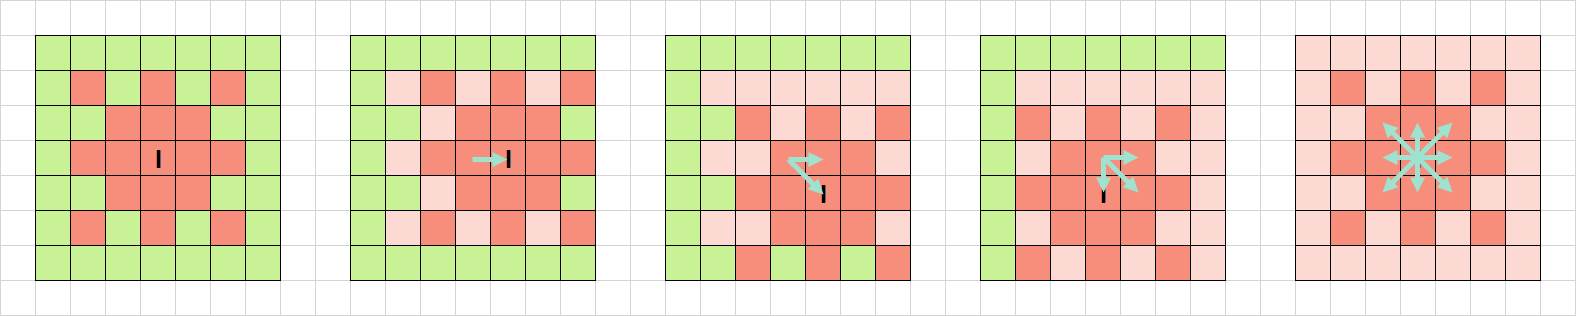
\includegraphics[width=1.0\textwidth]{screensAnalyse/fastRange}
\caption{Récupération du "carré" de portée d'une infanterie}\label{fig:analyse_fastcomp}
\end{figure}

\begin{figure}[H]
\centering
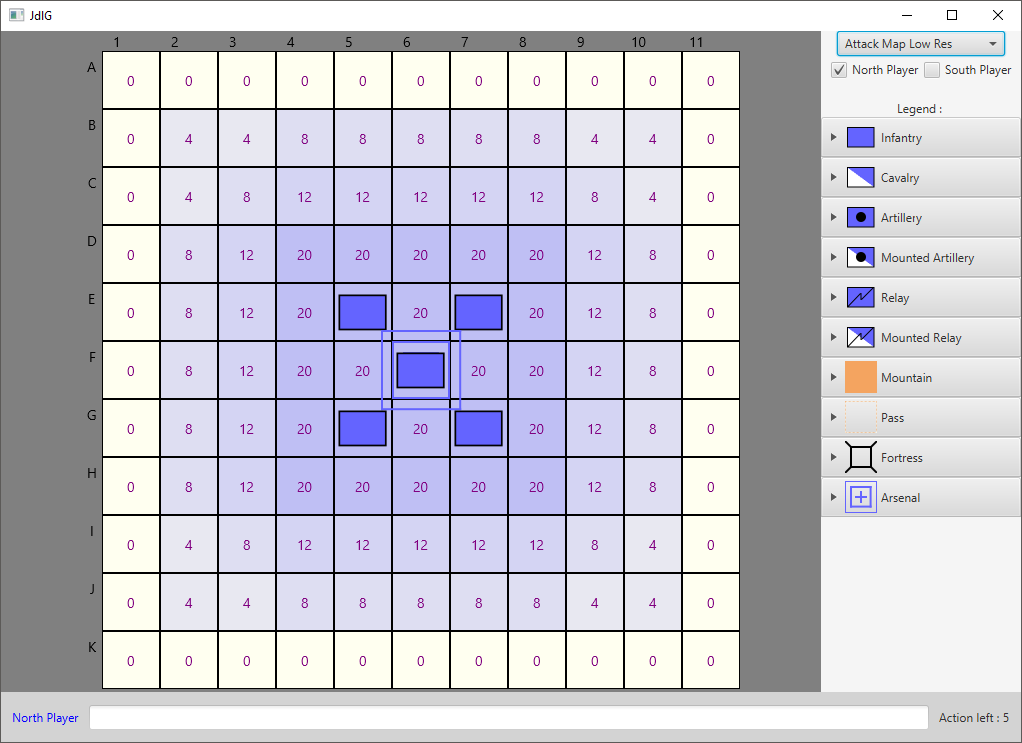
\includegraphics[width=0.9\textwidth]{screensAnalyse/attackStar}
\caption{Potentiel d'attaque d'une configuration "en étoile"}\label{fig:analyse_staratk}
\end{figure}

\begin{figure}[H]
\centering
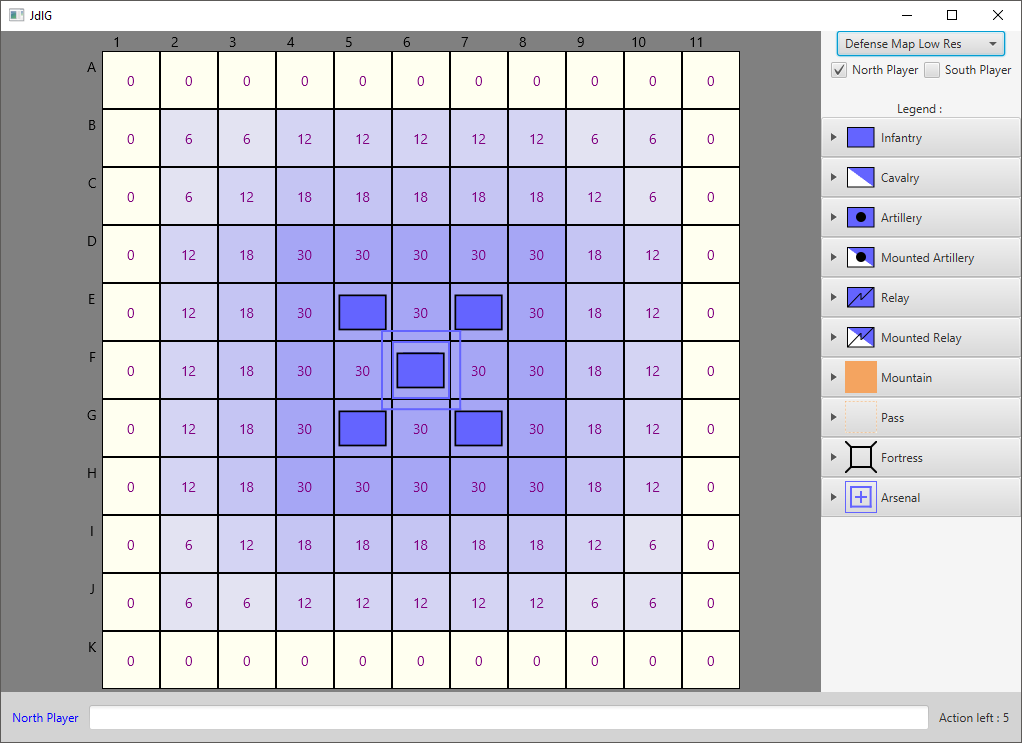
\includegraphics[width=0.9\textwidth]{screensAnalyse/defenseStar}
\caption{Potentiel de défense d'une configuration "en étoile"}\label{fig:analyse_stardef}
\end{figure}


\newpage

\subsection{Pistes d'exploitations possibles}
Les algorithmes implémentés sont largement améliorables : 


\paragraph*{} 
Le calcul de carte en comptant le déplacement d'une unité peut être étendu jusqu'à cinq coup, étant le nombre d'unités déplaçables par tour, donnant ainsi les meilleurs potentiels possibles, le tout de façon récursive. 

\paragraph*{} 
Les cartes d'attaques pourraient être "mémorisées" pour avoir des tuples \{positionnement, carte d'attaque\} pour pouvoir placer de façon optimiser un groupe d'unité pour attaquer une case en particulier, et de même pour la défense. Ces optimisations seraient tout aussi utiles pour un joueur humain que pour un joueur automatique.

\paragraph*{} 
Ces calculs demandant plus de performances, la prévision de coup pour un joueur automatique peut devenir problématique. Effectuer ces calculs sur une zone du plateau réduite pourrait aider à résoudre ce problème. Ainsi, on obtiendrait des calculs précis lors des affrontements (et donc utiles à la tactique), et on pourra utiliser des calculs moins précis, comme l'approche "rapide" décrite en \ref{sec:analyseEtoile}, pour avoir une idée générale de la situation du jeu (pour définir une stratégie).

\paragraph*{}
Une première configuration optimale a été remarquée plus tôt, et peut être utilisée pour influencer les coups à prendre pour un joueur artificiel, de même qu'une configuration pour se déplacer rapidement en un point critique, comme dans la partie présentée dans le livre de Debord, où un cavalier du camp Nord part attaquer seul un arsenal adverse. \`A l'inverse, ces configurations particulières pourraient aider à déterminer les intentions de l'adversaire et à les contrer de manière efficace.

\paragraph*{}
Le {\it Jeu de la Guerre} étant particulier pour son système de communications, l'analyse de ces lignes pourraient révéler un point "fragile" dans celles-ci et ce point deviendrait un objectif envisageable pour un joueur automatique afin d'affaiblir considérablement son adversaire. 

%%%%%%%%%%%%%%%%%%%%% TEST %%%%%%%%%%%%%%%%%%%

\chapter{Tests}
Les tests constituent une partie critique du projet. C'est eux qui nous permettent de nous assurer que le programme fait ce qu'on attend de lui à différents niveaux. Nous avons implémenté des tests unitaires, d'intégration et systèmes, à l'aide des bibliothèques {\it JUnit4} et {\it Mockito}.

Très peu de tests ont pu être effectués sur l'interface graphique de l'utilisateur, à cause de la difficulté à la rendre sous une forme exploitable et testable, comme le {\it XML} ou {\it SVG}. Nous ne nous sommes pas appuyés sur cette difficulté en raison de sa priorité moindre par rapport aux tests menés sur le reste de l'architecture.

\section{Les tests unitaires}
Les tests unitaires ont été implémentés au travers de différents scénarios, aussi bien valides qu'invalides, afin de tester nos méthodes en s'assurant ainsi qu'elles renvoient bien le résultat attendu. Pour chaque test de cas invalide, on vérifie que le message renvoyé pour signaler l'origine du problème est cohérent avec le problème provoqué. Le résultat des sous-règles dépendant généralement du contenu d'autres classes, à savoir \textbf{GameState} et \textbf{GameAction}, on utilise à la place des Mocks, ou "faux-objets", pour simuler leur comportement comme on le souhaite, donc en considérant le reste du programme comme infaillible. L'un des facteurs dont nous nous sommes le plus inspirés pour ces tests est la couverture de code, permettant de vérifier la pertinence du dit code.

\subsection*{Exemple : CheckIsChargeTest}

On effectue le test de la sous-règle \textbf{CheckIsCharge} en utilisant des unités de cavalerie et d'infanterie, représentant respectivement des unités avec la possibilité de charger et sans. On fait abstraction de la présence d'unités ennemies dans les cases ciblées, de la communication et des autres facteurs nécessaires à l'exécution d'une attaque car ce n'est pas dans le rôle de la règle testée de vérifier leur validité.

On tente de charger, avec une infanterie :
\begin{itemize}
\item Une case à proximité (Invalide).
\item Jusqu'au bout d'un alignement d'elle-même et de trois cavaleries (Invalide).
\item En participant à une charge menée par une autre unité de cavalerie (Invalide).
\end{itemize}

On tente de charger, avec 3 cavaleries alignées :
\begin{itemize}
\item Tel quel (Valide).
\item L'une des cavaleries de l'alignement ayant été forcée à battre en retraite (Invalide).
\item La cible n'est pas située au contact immédiat des cavaleries (Invalide).
\item La cavalerie initiant l'attaque positionnée dans une forteresse (Invalide).
\item Une autre cavalerie de l'alignement est positionnée dans une forteresse (Invalide).
\item La case ciblée contient une forteresse (Invalide).
\item La cavalerie initiant l'attaque est positionnée dans un col de montagne (Valide).
\item La case ciblée contient un col de montagne (Invalide).
\item L'une des cavaleries de l'alignement n'appartenant pas au joueur initiant l'attaque (Invalide).
\item La case cible n'est pas alignée avec la case de la cavalerie initiant la charge (Invalide).
\end{itemize}

\section{Les tests d'intégration}
Les tests d'intégration ont été imaginés afin de tester les interactions des classes et modules entre eux, c'est-à-dire cette fois sans utiliser de Mocks, en ayant le moteur de règles comme acteur principal. Certains de ces tests chargent des configurations spécifiques du plateau. Comme pour les tests unitaires, pour chaque cas invalide, on vérifie que le message retourné correspond à l'erreur provoquée.

\subsection*{Exemple : AttackRulesTest}

La liste des sous-règles impliquées dans la règle d'attaque est indiquée à la figure \ref{fig:treeAttack}, et la configuration de jeu utilisée est celle indiquée à la figure \ref{fig:boardAttack}. Ici, les tests doivent non seulement vérifier si une attaque est valide ou non, mais également que le résultat à l'issue de l'affrontement est correct, à savoir l'issue de cet affrontement, les valeurs d'attaque et les valeurs de défense calculées.

\begin{figure}[h]
\centering
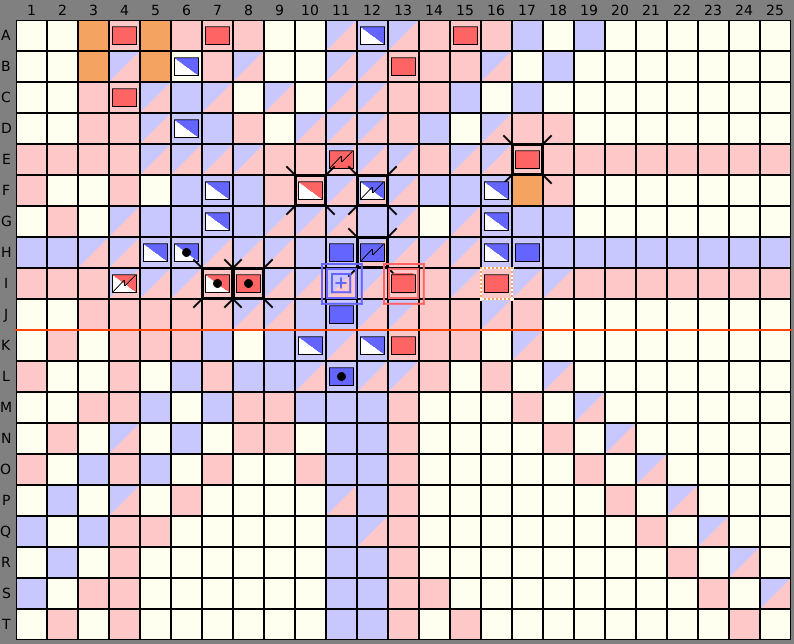
\includegraphics[width=0.85\textwidth]{tests/plateauAttaque}
\caption{Plateau de jeu des tests d'attaque}\label{fig:boardAttack}
\end{figure}

On vérifie les cas invalides :

\begin{itemize}
\item La case source de l'attaque ne contient pas d'unité alliée.
\item La case source de l'attaque contient une unité ennemie.
\item La case cible de l'attaque ne contient pas d'unité ennemie.
\item La case cible de l'attaque contient une unité alliée.
\item L'attaque n'a pas été précédée par un déplacement d'unité.
\item L'unité attaquante désignée n'est pas celle qui a effectué le dernier déplacement.
\item L'unité attaquante a déjà attaqué une fois à l'issue de son déplacement.
\item L'unité attaquante est une unité non combattante (unité relais).
\item La case ciblée par l'attaque est hors de portée de l'unité attaquante et il n'y a pas de charge possible entre ces deux positions. Ce cas est vérifié pour tous les types d'unités (sauf relais) et dans plusieurs configurations à la fois considérant la portée et la charge.
\item L'unité attaquante n'est pas alignée avec l'unité ciblée.
\item L'unité attaquante n'est pas alimentée en communication.
\item Il y a un obstacle empêchant l'unité attaquante de combattre l'unité ciblée.
\item L'unité attaquante a été forcée à battre en retraite.
\end{itemize}

Les tests valides étant nombreux, ils ne seront pas tous listés dans ce document. Il s'agit de vérifier en plus que les calculs d'attaque et de défense renvoient les bonnes valeurs, et que l'issue d'un combat (l'unité attaquée est intacte, doit battre en retraite, ou est détruite) est conforme aux valeurs renvoyées pour l'attaque et la défense.

\section{Les tests système}
Ces tests complètent les précédents, en s'assurant de la cohésion des éléments du jeu et en essayant de jouer une partie réelle via notre moteur de jeu. Ils s'effectuent sur le moteur de jeu et testent le plateau, le module système et le moteur de règles. Ces tests peuvent être étendus pour impliquer également l'interface utilisateur afin de jouer les coups en tant que joueurs "humain" et de tester le jeu dans son ensemble.

Étant donné que nous nous basons sur la partie et les règles du livre de Debord\cite{jdg}, notre test principal est joué sur des instances de la partie décrite. Cependant, des erreurs dans la partie illustrée dans le livre (voir section \ref{sec:Sujet} \nameref{sec:Sujet}) empêchent de jouer la partie dans son ensemble en suivant les règles et sans utiliser de moyen détourné (rajouter des tours factices permettant de jouer des coups autrement impossibles), nous avons décidé de n'en reproduire et de ne tester que quelques portions démontrant les aspects les plus importants du jeu. La partie elle-même ne présentant que certaines actions redondantes et peu de mécaniques, ces tests peuvent être complétés par des tests s'appuyant sur d'autres parties jouées afin de s'assurer que des parties plus complètes, plus complexes et moins erronées peuvent également être jouées.

Dans ces tests également, les configurations sont chargées à partir de fichiers (comme celle en figure \ref{fig:boardTurn42}) en début de test. Les actions (déplacement, attaque, fin de tour) sont jouées une par une et leur validité est vérifiée, et à chaque fin de tour un nouveau plateau est créé, permettant de vérifier manuellement qu'il correspond au résultat attendu. D'autres vérifications sont également possibles, par exemple dans le cas d'une attaque et destruction, on effectue une vérification avant l'attaque de la présence de l'unité attaquée à la case ciblée, et après l'attaque, de l'absence de cette même unité dans cette même case.

\begin{figure}[h]
\centering
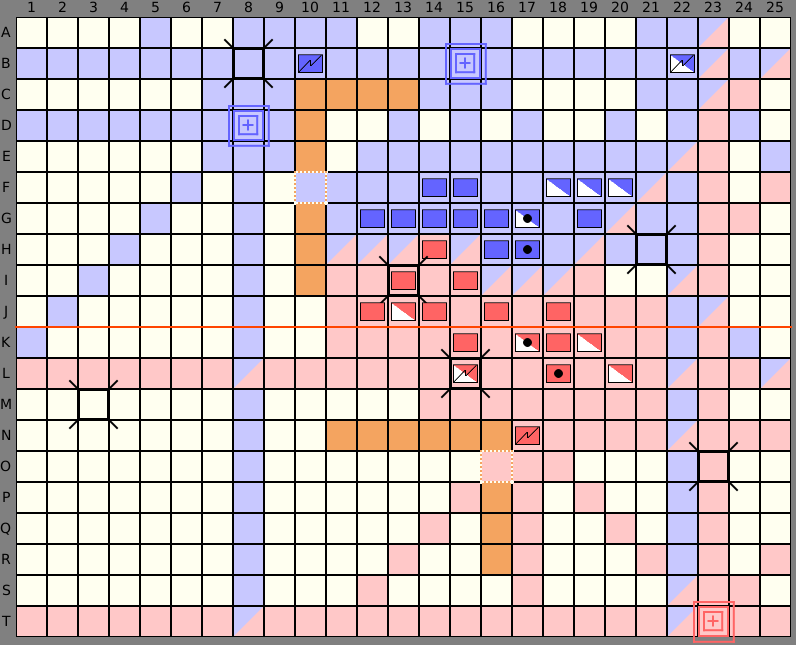
\includegraphics[width=0.85\textwidth]{tests/plateauTour42}
\caption{Plateau de jeu du tour 42 du livre}\label{fig:boardTurn42}
\end{figure}

\section{La couverture de code}

Le cœur du projet, le module de règles, est presque entièrement couvert (92\%), et seuls certaines des fonctions renvoyant des chaînes de caractères (comme {\tt toString()}), ainsi que certains renvois d'exceptions, ne sont pas couverts.

Le moteur de jeu et le déroulement du programme sont couverts à près de 80\% et le module d'analyse a également été couvert par des exemples de test.

Cependant, la partie interfaces utilisateur a été délaissée en raison de son implémentation (rendu graphiqueet synchronisation des threads).

\section{Tests des besoins}
Les points des besoins concernant l'affichage et l'interface graphique ne sont que très peu testés dans le projet, mais restent visuellement vérifiables sur l'interface graphique une fois une partie commencée.

\paragraph*{Besoins primaires}
La lecture, la traduction en coup des commandes écrites par l'utilisateur, la vérification de la validité des coups envoyés au jeu et l'application des coups validées sont bien testés et valides. De plus, la simulation de coup est très utilisée dans le module d'analyse, lui-même testé. La mécanique de changement de tour et d'alternance entre les deux joueurs est utilisée par les tests système et certains tests d'intégration.

\paragraph*{Besoins secondaires}
Le refus des coups et l'explication du refus sont vérifiés par les tests unitaires et d'intégration utilisant les règles, et les commandes de chargement et de sauvegarde de l'état du plateau, suivant la syntaxe définie, par les tests système.

Les extractions d'informations par le module d'analyse et le remplacement du joueur humain par un joueur automatique sont testables mais n'est pas couverts par nos tests.

\paragraph*{Besoins tertiaires}
Ceux-ci n'ont pas été implémentés et aucun test n'a été produit pour s'assurer de leur validité.

\paragraph*{Besoins non-fonctionnels}
Des tests de performance ont également été effectués, et le temps de réponse du moteur de règles à un coup proposé correspond aux besoins énoncés, et ces tests ont été réalisés à l'aide de \textit{profilers}.

\chapter{Conclusion}

\section{Perspectives et extensions}

\paragraph*{Aspect jeu}
Actuellement, le moteur de règles permet, à lui seul, d'altérer radicalement les règles du {\it Jeu de la Guerre}, cela peut être de la modification ou l'ajout d'unités, de terrain, des conditions de victoire, des méthodes de calcul pour la gestion de l'attaque, des déplacements ou même des communications.

Avec ce que nous avons et ce que nous permet le moteur de règles, nous pensons pouvoir implémenter d'autres jeux tour par tour sur plateau pouvant supporter plusieurs joueurs, comme les échecs, les dames ou encore le \textit{Reversi}.

Cependant, pour ce qui est d'une conversion totale du jeu, la liaison entre le moteur de règles et \textbf{GameState} est encore trop restreinte au {\it Jeu de la Guerre} pour obtenir un plateau de cases hexagonales par exemple (comme dans {\it DesertFox}), ou même sans cases (comme la série des {\it Warhammer}). Une conversion vers un genre de jeu avec une gestion plus profonde comme pour {\it DesertFox}, {\it Civilization} ou d'autres jeux de guerre reste possible mais à un degré assez limité. Par exemple, on peut implémenter une gestion de champ de vision ou de voie commerciale, de manière analogue aux communications, en modifiant de façon appropriée les {\it flags} dans \textbf{Board}. La conversion à un jeu d'une autre nature, comme un jeu de cartes ou un puzzle, est cependant difficilement envisageable : il serait préférable de refaire un moteur de règles ayant comme objectif d'être adaptable à n'importe quel jeu plutôt que de modifier celui-ci.

En soi, le moteur de règles possède un degré de généricité étendu pour un jeu au tour par tour à plusieurs joueurs, avec ou sans plateau. Afin de pouvoir être exploité au maximum, il aurait fallu rendre \textbf{GameState} et \textbf{Board} bien plus génériques qu'ils ne le sont actuellement, mais cela sort des objectifs de ce projet.

En ce qui concerne le \textit{Jeu de la Guerre}, il reste à implémenter les règles d'initialisation de la partie, comme le positionnement des bâtiments et des unités tout en cachant les effectifs adverses, ainsi que pour déterminer le joueur qui débutera la partie.

Aussi, il faudrait implémenter une règle permettant de s'assurer qu'une instance du plateau respecte bien les conditions décrites dans le livre, par exemple les forteresses sur des cases en liaison directe avec ses arsenaux, le nombre de montagnes ou encore l’asymétrie du plateau. Le reste des règles est implémenté, testé et fonctionne dans l'exécutable produit.

\paragraph*{Système expert}

Concernant un système expert, comme nous l'avons décrit dans les parties précédentes, nous avons une première implémentation d'un joueur automatique ainsi qu'un module d'analyse. Actuellement, nous calculons principalement des cartes d'attaques et de défenses de chaque camps en prenant en compte un et aucun déplacement, ainsi que des déplacements valides d'unités.

Actuellement notre joueur automatique n'utilise que la génération des déplacements valides afin d'en jouer un au hasard. Nous avons pensé à diverses pistes afin de rendre ses déplacements plus cohérents.

Tout d'abord nous avons pensé à trier la liste des déplacements possibles par le nombre total de cases en communication que ça engendrerait, et de choisir parmi les 10\% meilleurs résultats un mouvement au hasard. Cela pourrait peut-être faire apparaître des positionnements d'unités plus favorables permettant de favoriser la communication lors de déplacement. Une autre façon d'aborder ce cas pourrait être de trier les déplacements en fonction du nombre de déplacements valides qui serait possible d'effectuer à la suite du déplacement, ainsi cela favoriserait une plus grande liberté de mouvement.

De manière analogue en utilisant les cartes d'attaques/défenses, privilégier les déplacements qui permettent de conserver un maximum de potentiel d'attaque ou de défense lors de déplacement, et à l'issue de ce déplacement avoir une liste des attaques possibles qui permettent la retraite ou la destruction d'une unité ennemie.

\paragraph*{Stratégies applicables au \textit{Jeu de la Guerre}}

Lors de nos différentes parties sur le jeu, nous avons pu constater quelques stratégies qui pourraient être applicable à un système expert.
Nous détaillerons dans cette partie les différentes stratégies que nous avons pu remarquer.

Tout d'abord une première stratégie, qui se trouve appliquée dans les premiers tours de la partie décrite dans le livre, pourrait être de focaliser ses forces vers les arsenaux ennemis à l'aide d'unités rapides.

Un autre plan que pourrait utiliser le système expert serait d'affiner la stratégie précédente en calculant les faiblesses dans la formation des unités ennemies permettant au joueur automatique de mieux déplacer ses unités afin d'atteindre plus facilement les arsenaux.

Une autre stratégie envisageable serait de jouer sur la défensive, et donc de privilégier la protection de ses arsenaux et de ses unités relais afin de forcer l'ennemi à attaquer.

L'utilisation des cartes d'attaque et de défense semble cruciale pour déterminer les mouvements globaux des troupes, et en garder une trace pourrait permettre de mieux discerner les intentions de l'ennemi pour plus facilement le contrer.

\paragraph*{Bilan}

Nous pensons avoir atteint la majorité des objectifs que nous nous étions fixés, mais avons manqué de temps pour tous les réaliser.

La phase d'initialisation de la partie n'a pas du tout été implémentée, et nécessiterait en plus de l'ajout de quelques règles une modification de la classe \textbf{Game}. En l'état, cette classe n'est pas capable de gérer des étapes au cours d'une partie.

Nous n'avons pas non plus implémenté de stratégie pour permettre au système expert de pondérer l’intérêt d'un coup, celui-ci le choisissant donc aléatoirement. Des recherches on néanmoins étés faites sur ces stratégies, que nous détaillons en section \ref{sec:analyse}.

Finalement, réaliser ce projet nous a appris de nombreuses choses sur la manière de mener le développement d'un logiciel. Le temps que nous avons passé a réfléchir au projet avant de commencer le développement nous a permis de mieux commencer la phase de code, nous a permis d'éviter d'erreurs de conceptions qui auraient pu gravement nuire au futur développement, ce qui à terme nous a conduit à avoir des bases plus solides que lors des projets précédents que nous avions pu faire.

Nous avons également appris à nous servir de différents outils pour nous aider dans notre tâche, tels que Doxygen avec lequel nous avons pu nettement améliorer l'organisation de notre code, ou encore de profilers.

Enfin, nous espérons que le travail conduit au cours de ce projet pourra être réutilisé par d'autres groupes de Projet de Programmation dans les années à venir.

%
% ---- Bibliography ----
%
\nocite{*}
\printbibliography[
heading=bibintoc,
title={Bibliographie}
]



\setlength{\parskip}{0.0em}
\listoffigures
\setlength{\parskip}{0.5em}

\appendix
\chapter{}
\centering
\begin{lstlisting}[basicstyle=\scriptsize\tt, columns=fullflexible, caption=Fichier pour l'état initial présenté dans le livre \it{Le Jeu de la Guerre},label=lst:formatDebord]
25;20
1;5
F;8;2;1
F;21;8;1
F;13;9;1
AR;15;2;1
AR;8;4;1
M;10;3;1
M;10;4;1
M;10;5;1
M;10;7;1
M;10;8;1
M;10;9;1
M;11;3;1
M;12;3;1
M;13;3;1
CO;10;6;1
F;3;13;2
F;15;12;2
F;23;15;2
AR;3;20;2
AR;23;20;2
M;11;14;2
M;12;14;2
M;13;14;2
M;14;14;2
M;15;14;2
M;16;14;2
M;16;16;2
M;16;17;2
M;16;18;2
CO;16;15;2
R;3;4;false;true;false;true;1
RC;5;6;false;true;false;true;1
C;3;7;false;true;false;true;1
C;4;7;false;true;false;true;1
C;3;8;false;true;false;true;1
C;4;8;false;true;false;true;1
I;5;8;false;true;false;true;1
I;10;6;false;true;false;true;1
I;6;7;false;true;false;true;1
I;7;7;false;true;false;true;1
I;9;7;false;true;false;true;1
I;7;8;false;true;false;true;1
I;8;8;false;true;false;true;1
I;9;8;false;true;false;true;1
I;6;9;false;true;false;true;1
A;8;7;false;true;false;true;1
AC;6;8;false;true;false;true;1
R;23;15;false;true;false;true;2
RC;17;14;false;true;false;true;2
C;19;11;false;true;false;true;2
C;19;12;false;true;false;true;2
C;18;12;false;true;false;true;2
C;18;13;false;true;false;true;2
I;15;11;false;true;false;true;2
I;15;12;false;true;false;true;2
I;15;13;false;true;false;true;2
I;16;11;false;true;false;true;2
I;16;12;false;true;false;true;2
I;16;13;false;true;false;true;2
I;17;11;false;true;false;true;2
I;17;12;false;true;false;true;2
I;17;13;false;true;false;true;2
A;18;11;false;true;false;true;2
AC;16;15;false;true;false;true;2
\end{lstlisting}

\end{document}

